\ac{COD} is one of the most important variables in the process of a biological treatment since experts can make decisions based on the measurements of this variable. The objective of biological wastewater treatment is to perform a removal of the pollutants present in water. Thus, this treatment is used overall because it is compelling and more efficient than numerous mechanical or compound procedures. In the bioreactor at this stage, a variety of microorganisms are used to break down organic matter in the water. However, the microorganisms are susceptible to change, depending on several the bioreactor conditions. Likewise, it results relevant monitoring the concentration of biomass available in the bioreactor which indicates the state of the microorganisms population.

This study proposes to predict one-day time-window \ac{COD}\textsubscript{D}, \ac{COD}\textsubscript{EQ}, and \ac{MLVSS}, essential parameters in decision-making, knowing how contaminated the water will be at the effluent stream (discharge point), the organic matter concentration at the input of the bioreactor, and how the microorganism population in charge of the biological stage is going to behave. 

\begin{figure}[h]
\centering
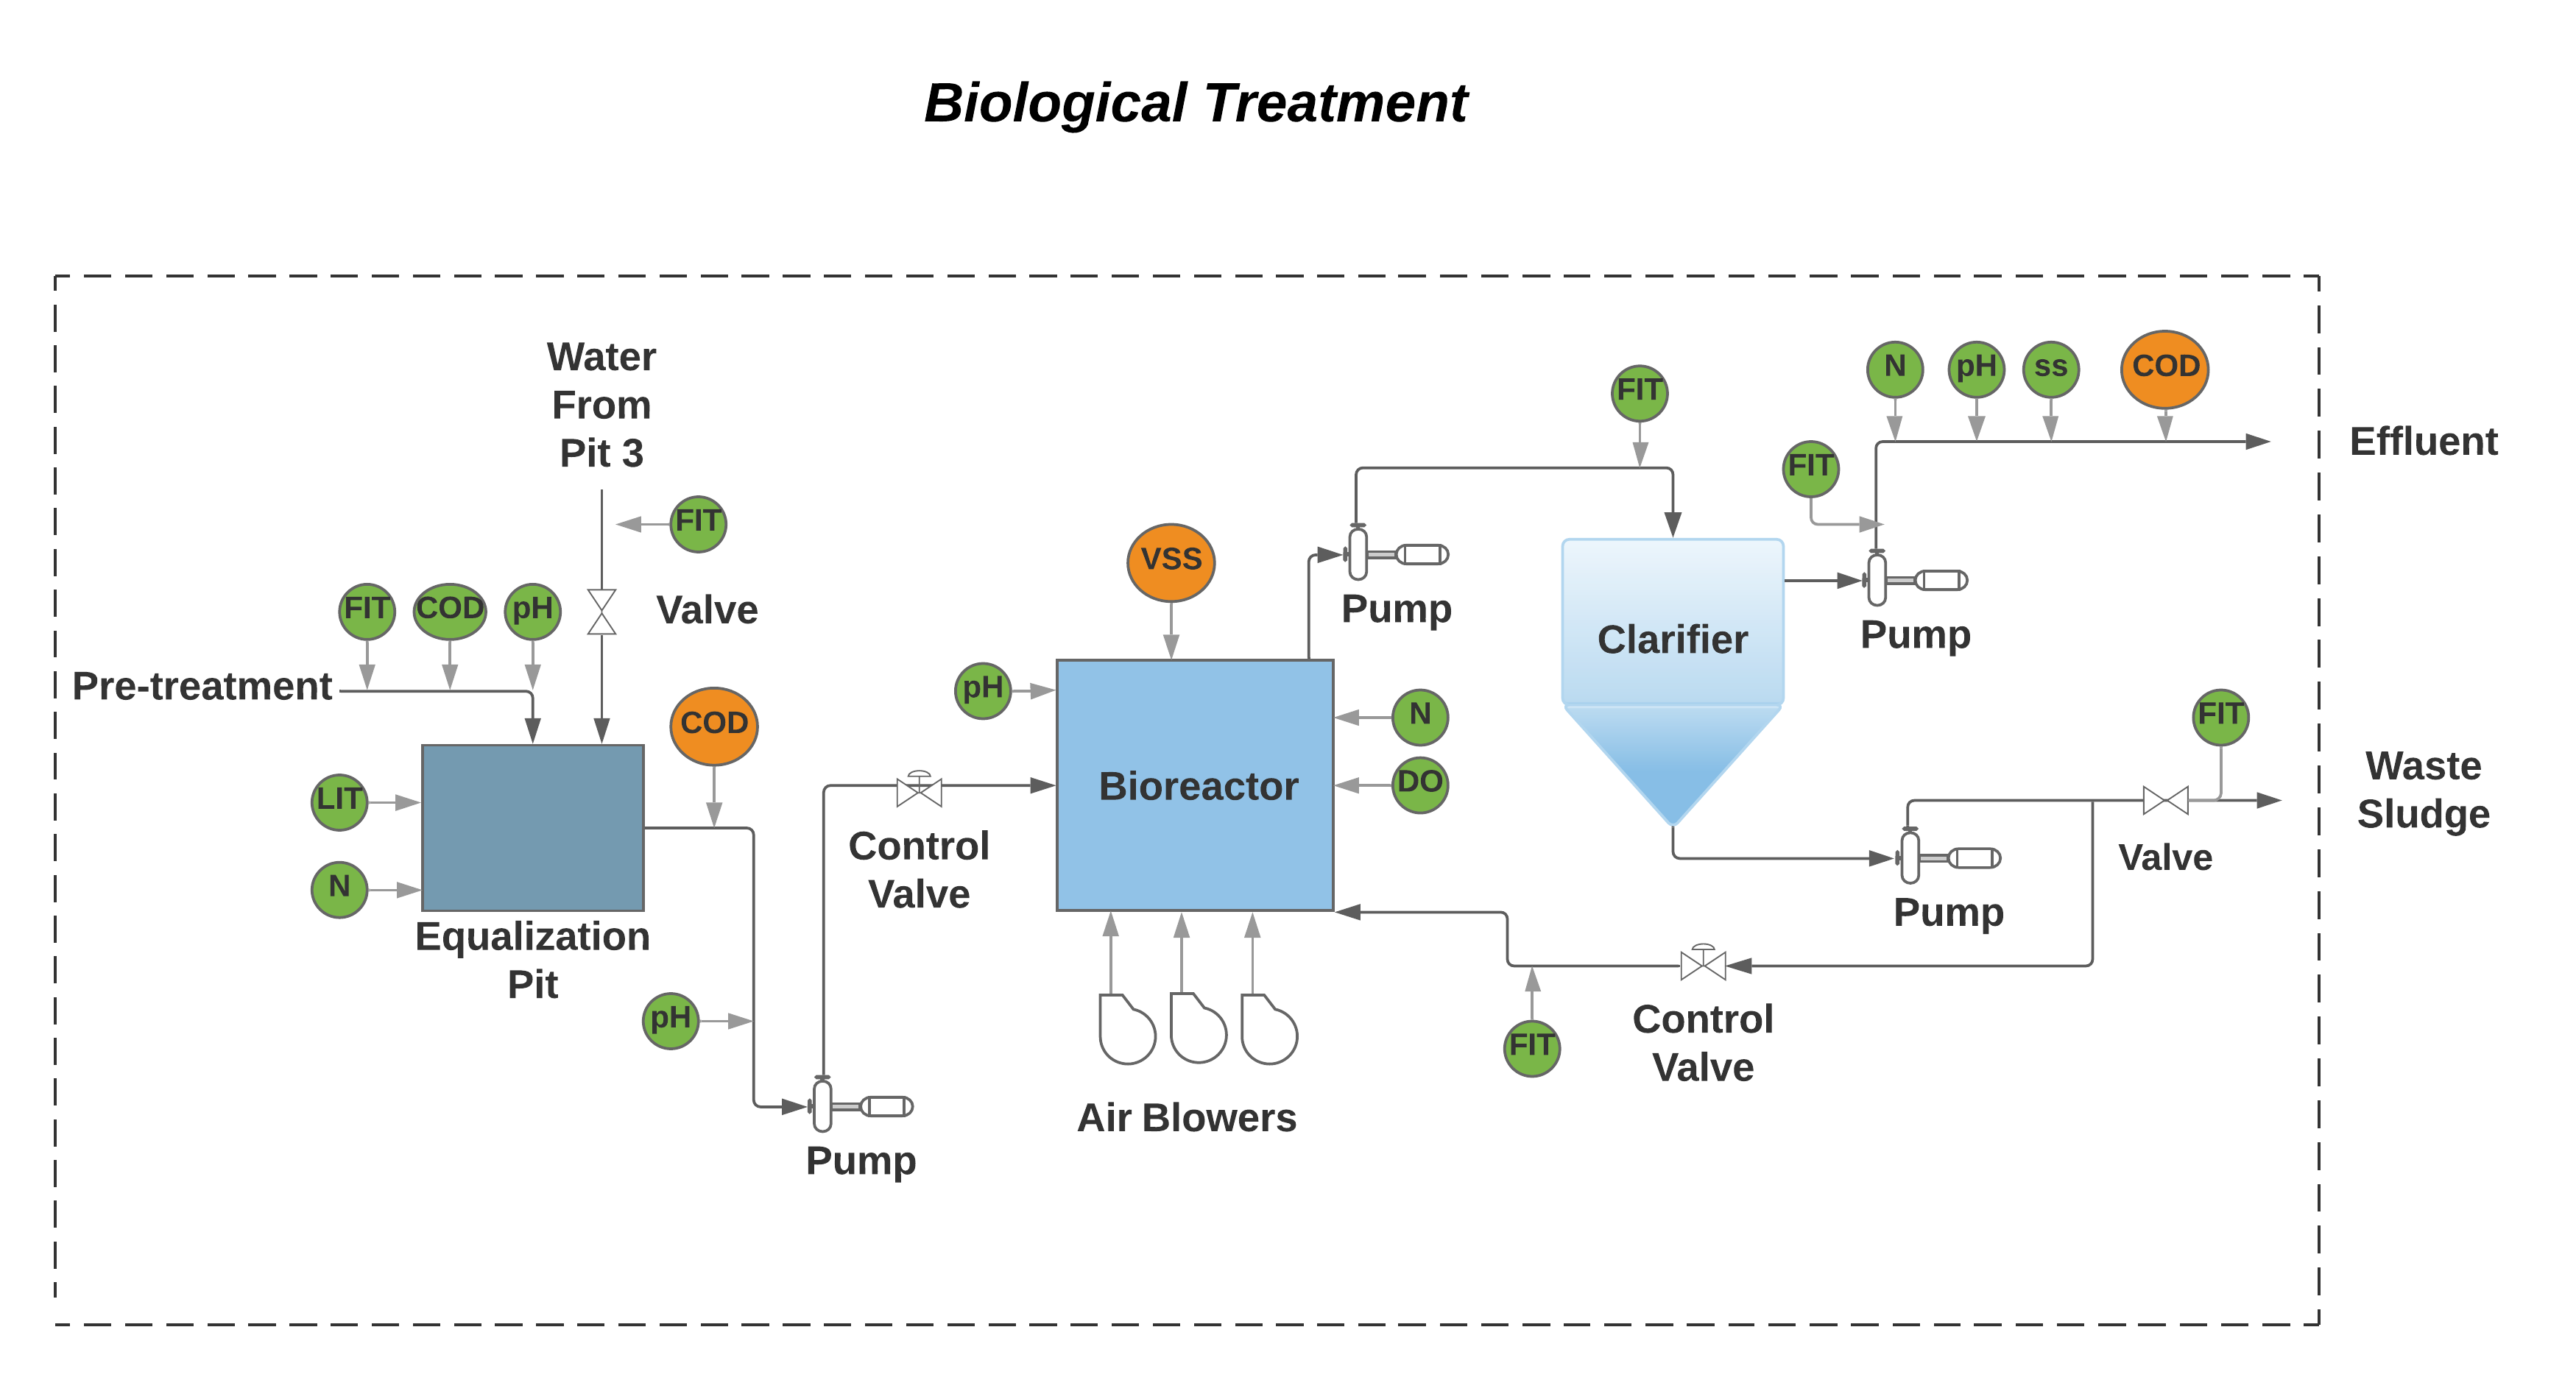
\includegraphics[width=\linewidth]{figures/Ch4/Biological-treatment-stage.png}
\caption{Biological Treatment Stage}
\label{f:Biological-treatment}
\end{figure}

\autoref{f:Biological-treatment} illustrates the composition of the biological treatment stage which is the case of study in this research. The stage has three main components and each one plays an important role in the organic load removal, an equalization pit, a bioreactor, and a clarifier. Green circles represent measured variables of interest and potential input variables for the system. Orange circles are the target variables of this work, which are also available.

This work uses python programming language to implement the intelligent system, supported by several libraries such as Numpy, Pandas, Tensor Flow, Sci-kit Learn, Matplotlib, among others. A GitHub repository contains the files corresponding to code, models, and some of the results presented in this document \footnote{\url{https://github.com/carloscp3009/Machine-Learning-Approaches-for-Industrial-data-forecasting}}. 

The study utilizes 343 data samples from a wastewater treatment facility located in Nantong, China. Measurements correspond to most of the year 2018 and present a daily frequency, which experts consider accurate to capture the process dynamics. The measured variables of the process available for this work are:

\begin{itemize}
 \item	Flow
 \item	COD of influent water
 \item	Suspended solids in influent water (SS)
 \item	Mixed liquor suspended solids (MLSS)
 \item	Mixed liquor volatile suspended solids (MLVSS)
 \item	Nitrogen (N)
 \item	pH
 \item	Mixed liquor dissolved oxygen (DO)
 \item	Food to microorganism (F/M)
\end{itemize}

The following nomenclature determines the unit process or component within the biological stage that the variable is measured.

\begin{itemize}
 \item	EQ = Equalizer
 \item	BIO = Bioreactor
 \item	BT\textsubscript{N}= Bioreactor Pit N
 \item	BT\textsubscript{C}= Bioreactor Pit C
 \item	Clari = Clarifier
 \item	OxT = Oxidation Tank
 \item	D = Discharge Pit
\end{itemize}

%\begin{longtable}{@{}l *{2}{rr}}
\begin{longtable}[h!]{@{}l *{2}{rr}}
\caption[Portrait Table, short caption]{Variables Correlation}
\label{t:correlation_table}
\\
%   
\toprule%


 {\bfseries Variable} & {\bfseries COD\textsubscript{D} } & {\bfseries COD\textsubscript{EQ}} & {\bfseries MLVSS}
\\

\cmidrule[0.4pt](r{0.125em}){1-1}%
\cmidrule[0.4pt](lr{0.125em}){2-4}%
%\cmidrule[0.4pt](lr{0.125em}){4-5}%
%\cmidrule[0.4pt](lr{0.125em}){5-6}%


  \endfirsthead

\endhead

        Flow\_to\_EQ & 0.14 & -0.14 & -0.025  \\ 
        BT\_C\_MLSS & 0.11 & -0.43 & 0.88  \\ 
        BT\_C\_MLVSS & 0.10 & -0.45 & 0.9  \\ 
        BT\_N\_MLSS & 0.10 & -0.44 & 0.88  \\ 
        BT\_N\_MLVSS & 0.10 & -0.44 & 0.88  \\ 
        D\_SS & 0.3 & 0.59 & -0.46  \\ 
        EQ\_N & 0.25 & 0.74 & -0.54  \\ 
        BT\_C\_N & 0.25 & 0.49 & -0.54  \\ 
        BT\_N\_N & 0.11 & 0.26 & -0.47  \\ 
        D\_N & 0.11 & 0.23 & -0.46  \\ 
        OxT\_pH & -0.12 & -0.33 & 0.27  \\ 
        EQ\_pH & -0.069 & 0.18 & -0.17  \\ 
        BT\_N\_pH & 0.057 & -0.045 & 0.083  \\ 
        D\_pH & 0.059 & -0.13 & 0.078  \\ 
        BT\_N\_DO & -0.1 & -0.37 & 0.14  \\ 
        BT\_C\_DO & -0.28 & -0.33 & 0.34  \\ 
        Clari\_DO & -0.17 & -0.43 & 0.27  \\ 
        ST\_COD & 0.22 & 0.63 & -0.44  \\ 
        D\_COD\_ON & 0.72 & 0.22 & 0.11  \\


\bottomrule

\end{longtable}
\autoref{t:correlation_table} presents the Person correlation of the three target variables this study cover. The correlation coefficient allows to select the exogenous variables used as inputs for the system. This enhances the model learning capability by reducing the noise of not correlated variables and decreasing the number of trainable parameters which implies a model complexity reduction. 

After variable selection, the dataset is split into training (0.8), validation (0.1) and test (0.1) sets. The first 80\% of the dataset serves as examples for the model to learn, the following 10\% allows to validate the model performance for early stopping, and hyper-parameters tuning, and the last 10\% is used to evaluate the performance of the model using new data, this way obtaining a certainty of its behaviour in production mode. 

It is important to note that a computational technique must be selected. As mentioned before in related works in \autoref{t:state-of-art}, about 64.71\% of the work of authors used an algorithm from the ANN group to develop forecast models. It has been verified that neural networks have suitable results in the area since the water treatment process is characterized by being nonlinear, so if they are used properly, they can represent the dynamics of this process very well. 

Once a technique is selected, the training of the model begins. An error measure is necessary to support the performance of the model. Therefore, defined as shown in \autoref{eq:MAPE} is used as the evaluation metric.

\begin{figure}[h]
\centering
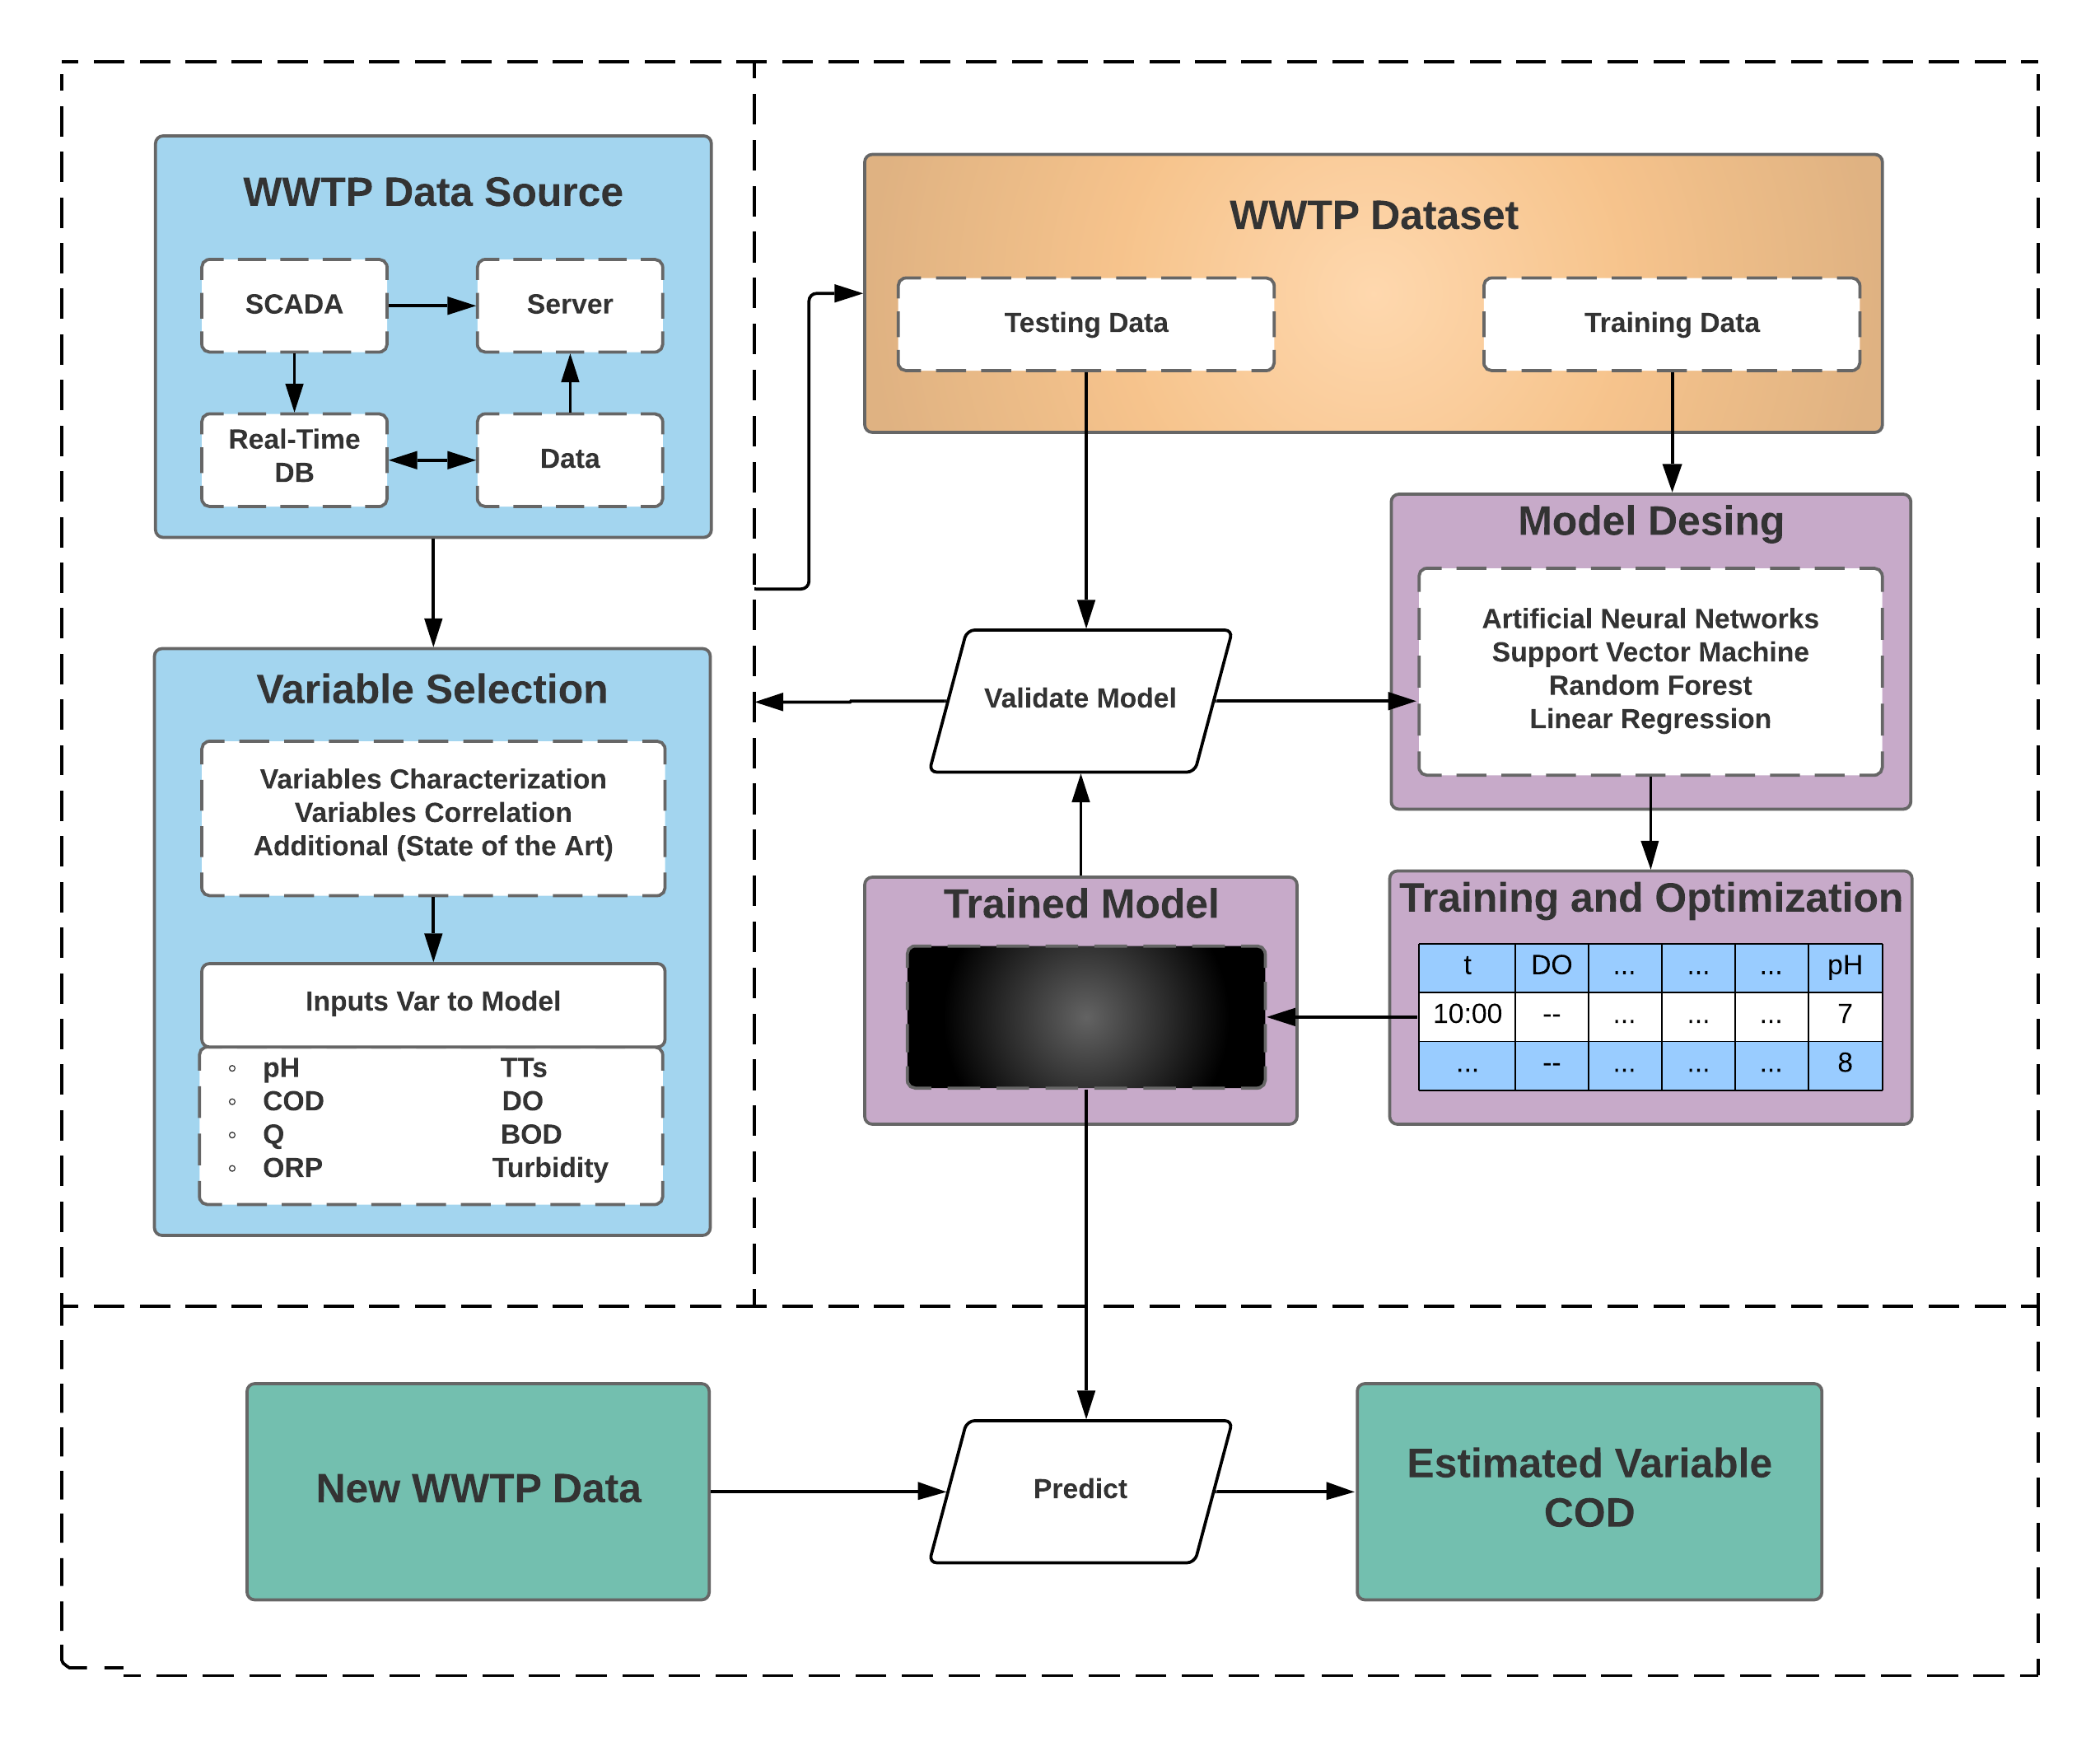
\includegraphics[width=\linewidth]{figures/Ch4/training-FlowChart.png}
\caption{Traininf flow chart}
\label{f:training-flowchart}
\end{figure}

\section{Approach 1}
\label{s:Approach1}

\autoref{f:Approach 1} shows in more detail how the model is conceived and how the COD forecasting is achieved. First, the objective variable taken from the dataset is studied using a time-series decomposition technique that transforms the variable into three additive components: trend, seasonality and residual. Leveraging an auto correlation study over the components, the first two are estimated using their past values. On the other hand, the residual component is estimated using an ANN, which received exogenous variables selected from a correlation study and a past value of the same component. Finally, the addition of the three components provides the COD prediction. 

\begin{figure}[h]
\centering
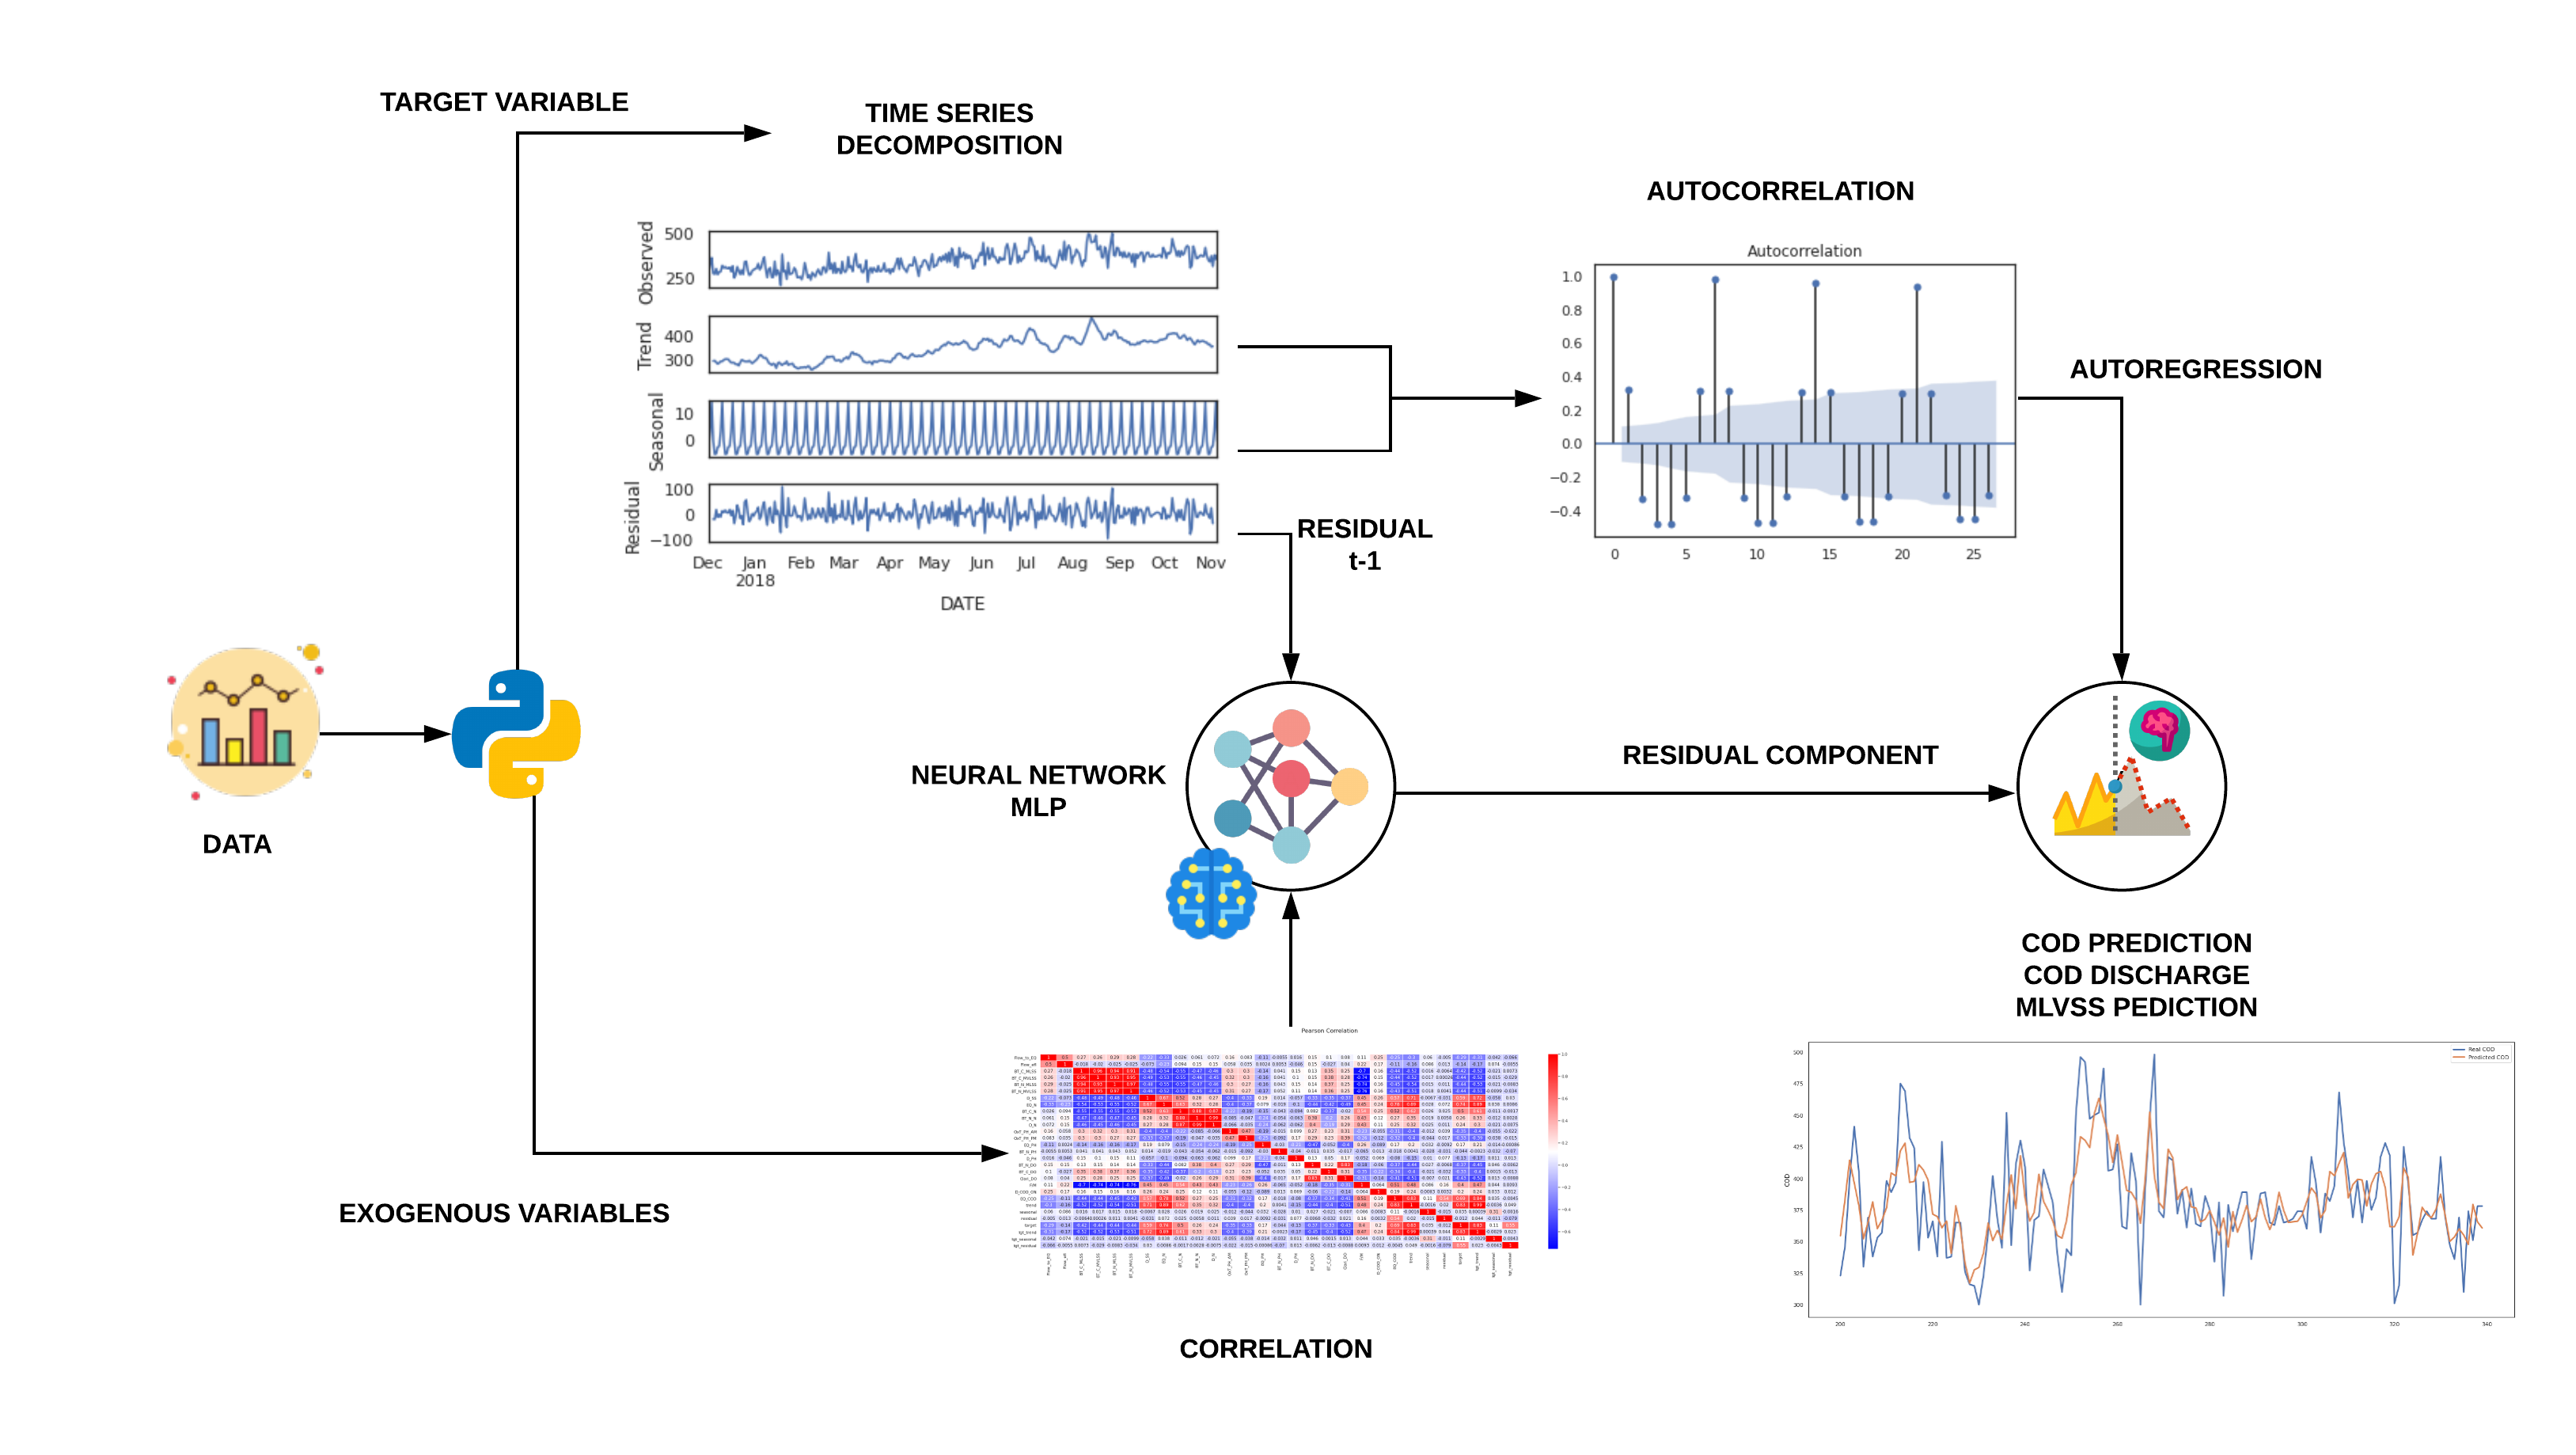
\includegraphics[width=\linewidth]{figures/Ch4/Approach1.png}
\caption{Approach 1}
\label{f:Approach 1}
\end{figure}

\subsection{Time Series Decomposition}
For the time-series analysis of the target, the variable was made a component decomposition where the time series could be represented as a combination of trend, seasonality and residual components [35]. From this point, it was intended to forecast each component of the time series to obtain the objective series using the additive model stated by Pearson and presented in Equation (2) [36], where Tt refers to tendency or trend, St to seasonal movements, Rt to residuals or irregulars and Xt to the series observed.

Figure 7 shows an example of how the equalizer’s COD decomposition looks for the year 2019, where (a) shows the original COD variable, (b) the trend component, (c) the seasonal component and (d) the residual component.

\begin{figure}[h]
\centering
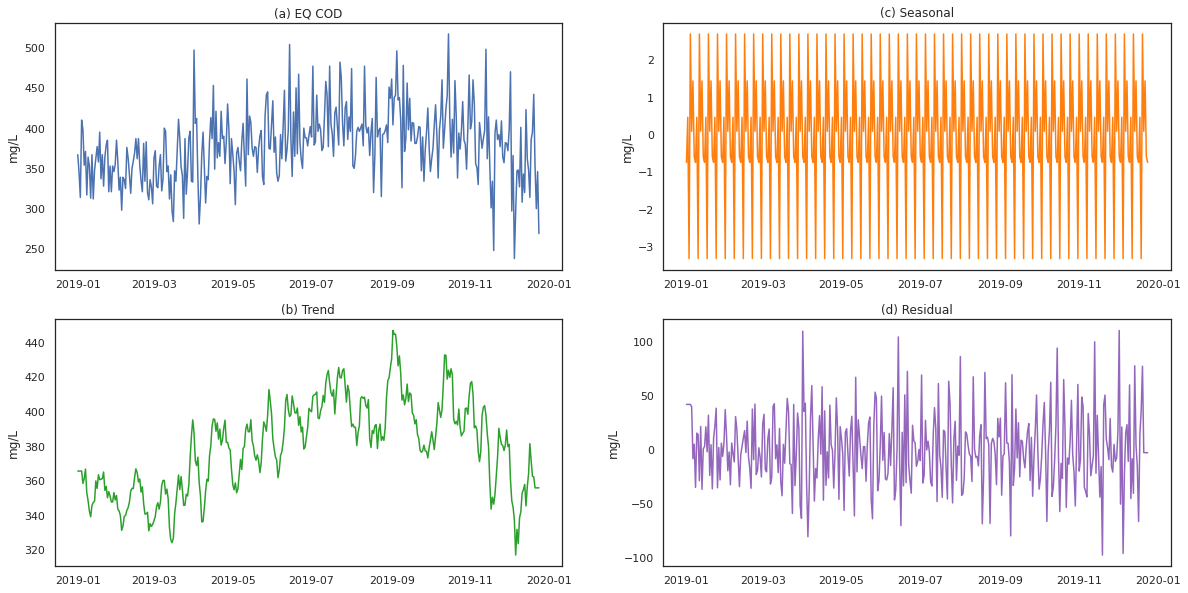
\includegraphics[width=\linewidth]{figures/Ch4/time_series_descompose.png}
\caption{Time Series Decomposition}
\label{f:Time-series-decomposition}
\end{figure}

\subsection{Autocorrelation Study}
Analyzing the time-series decomposition, both autocorrelation and partial autocorrelation studies were made on residual, seasonal and trend COD to extract the important characteristics. From this analysis, it was possible to conduct an autoregressive estimation of the trend and seasonal component of the series. Figures 8, 9, and 10 show the total and partial autocorrelation, respectively. 
\subsection{Model Design}

\newpage
\begin{figure}[h]
\centering
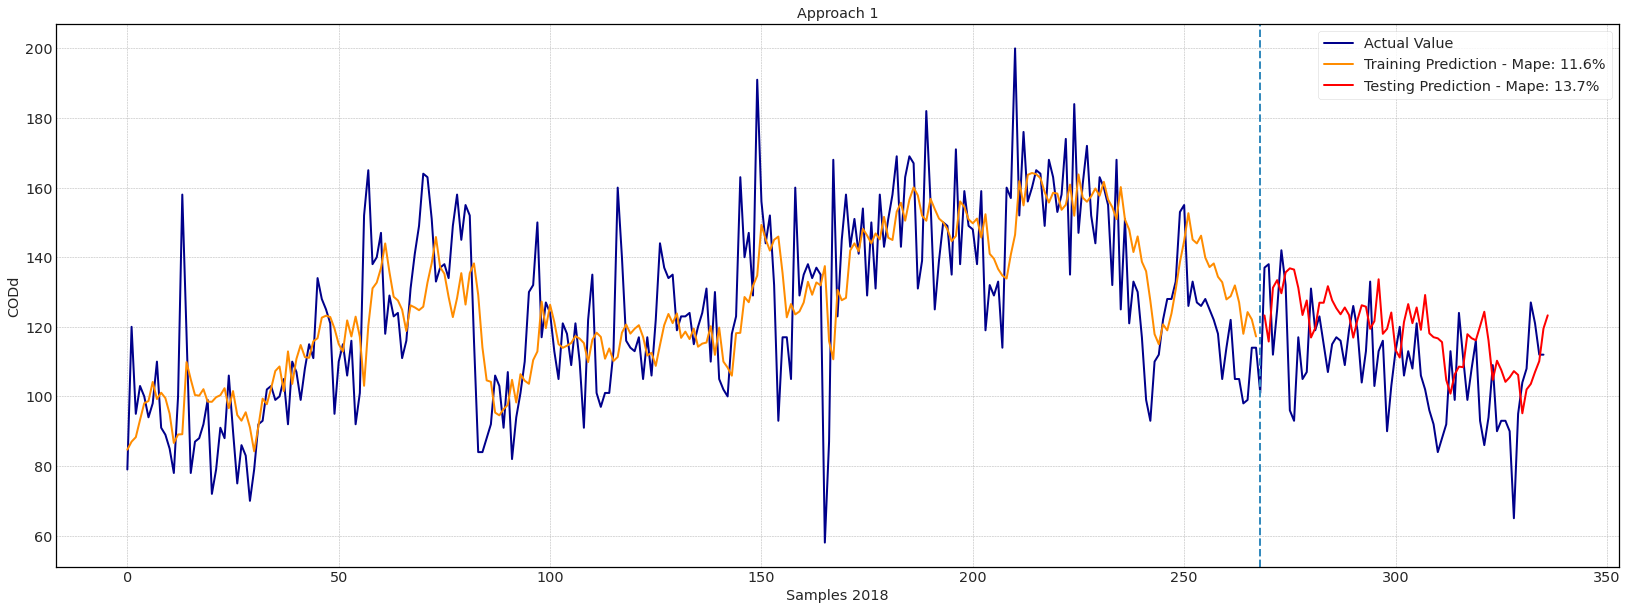
\includegraphics[width=\linewidth]{figures/Ch4/CODd-1.png}
\caption{Approach 1 - CODD}
\label{f:App1-codd}
\end{figure}

\begin{figure}[h]
\centering
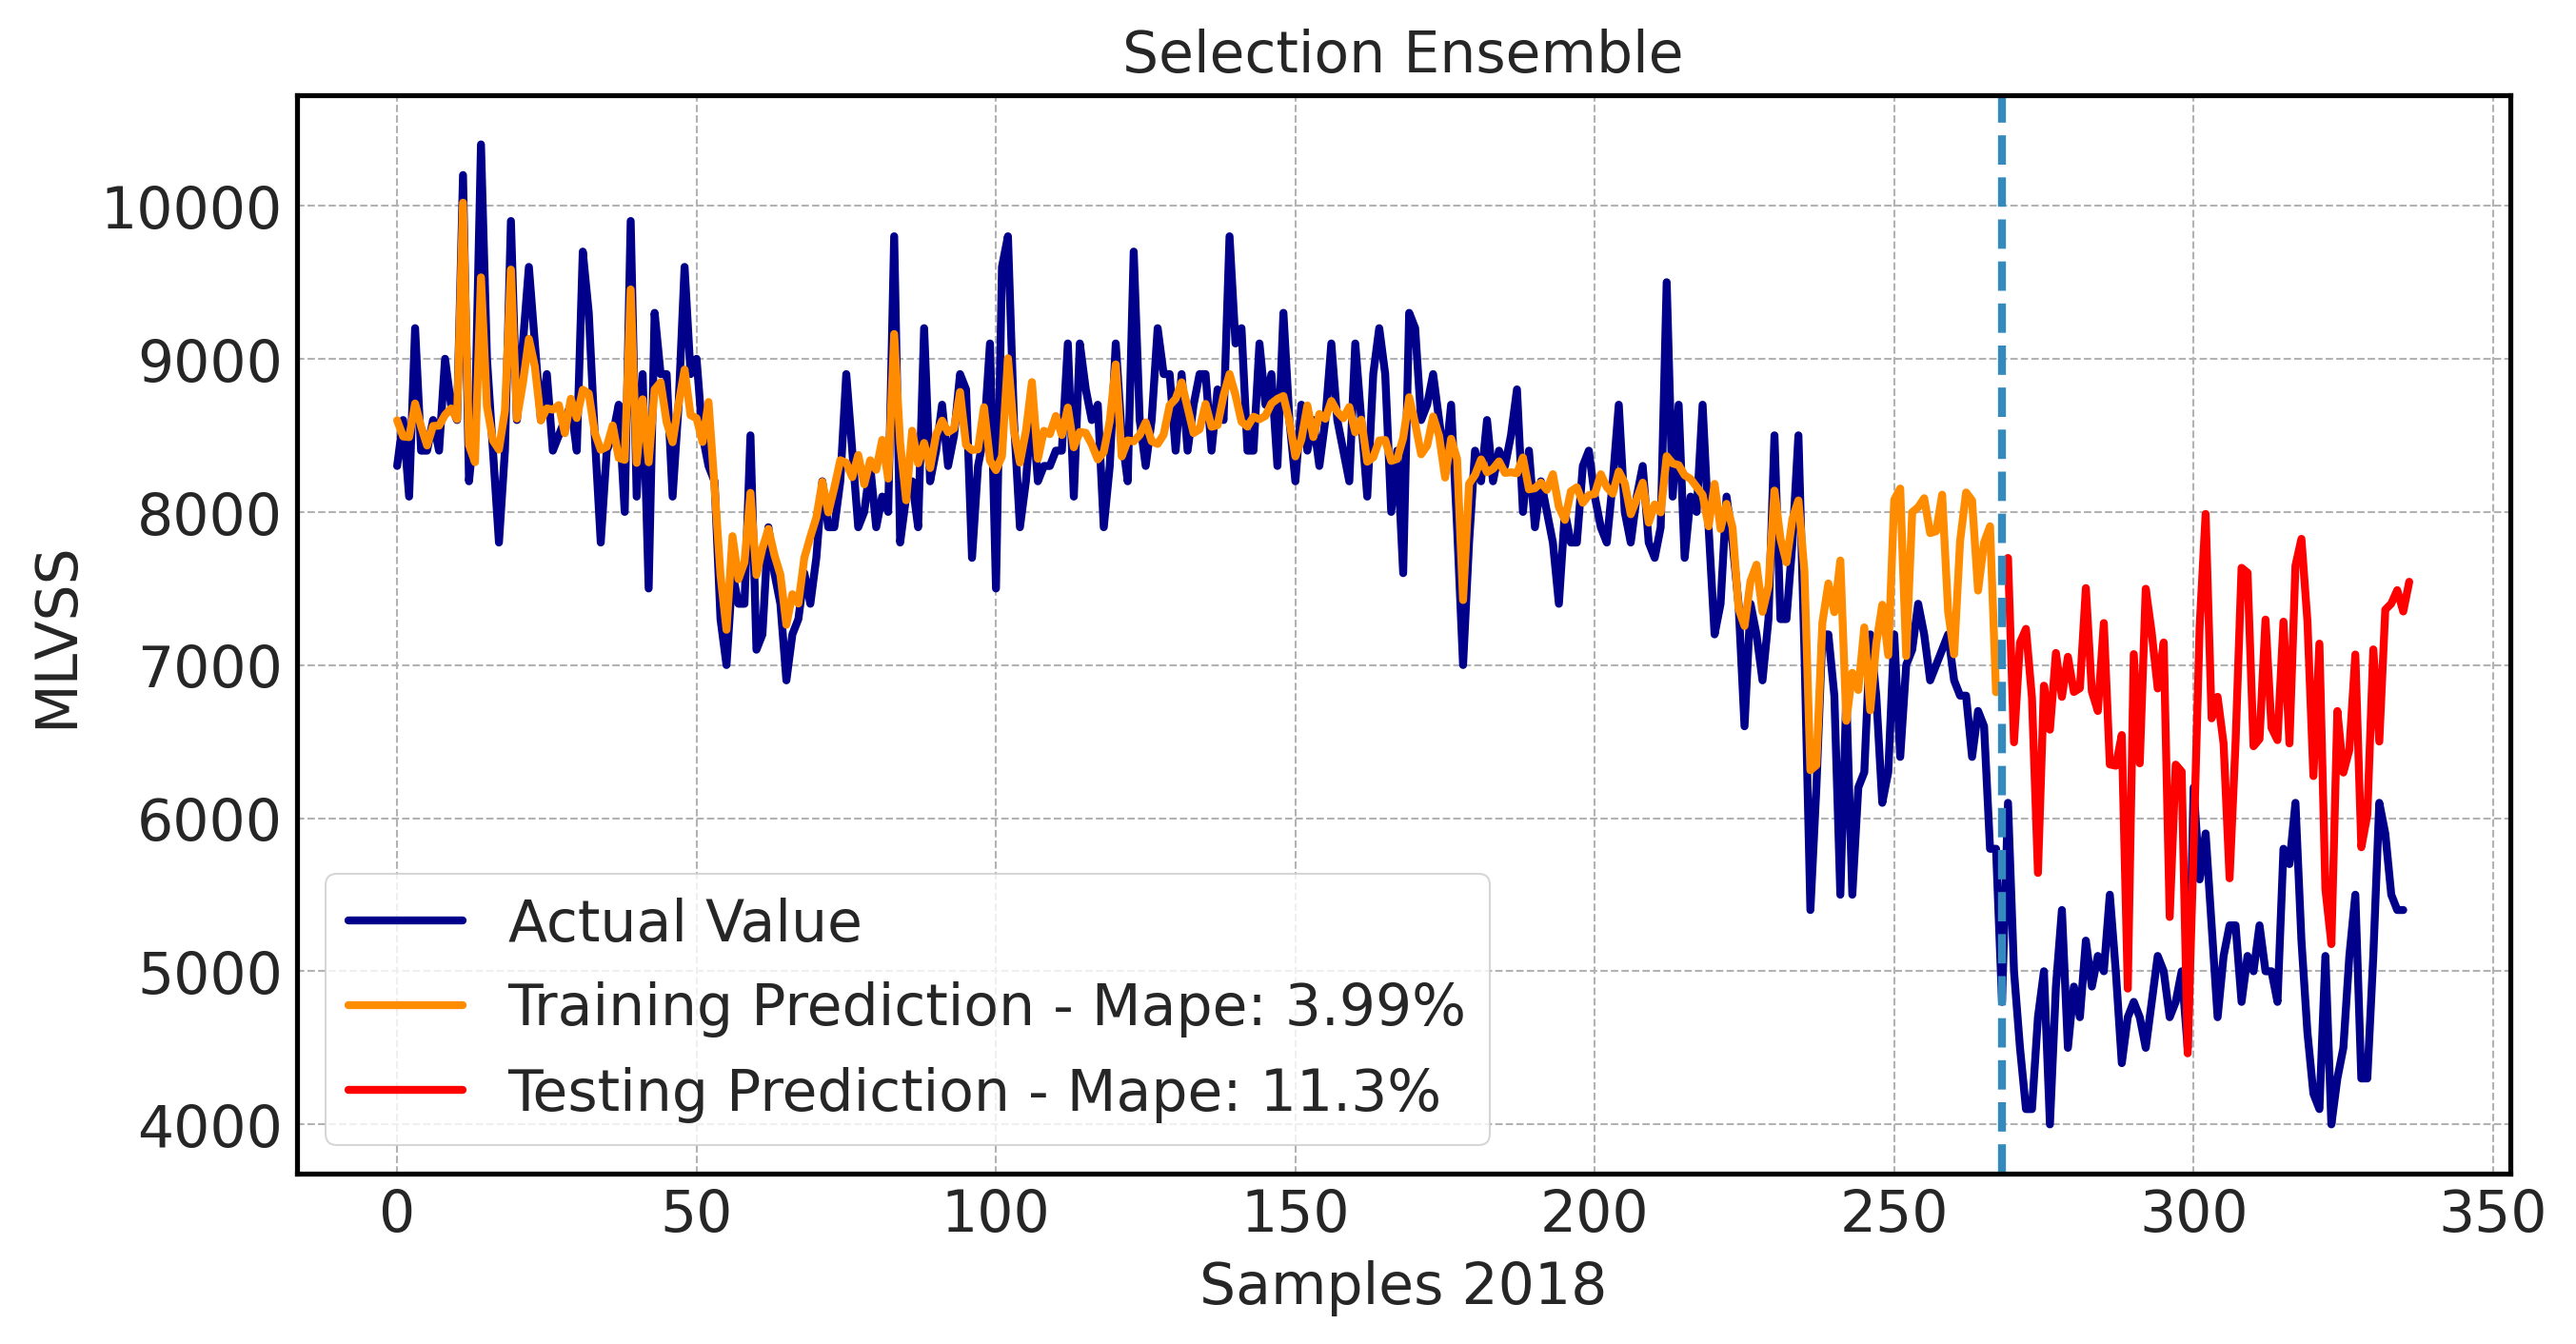
\includegraphics[width=\linewidth]{figures/test2.png}
\caption{Approach 1 - CODEQ}
\label{f:App1-codeq}
\end{figure}

\begin{figure}[h]
\centering
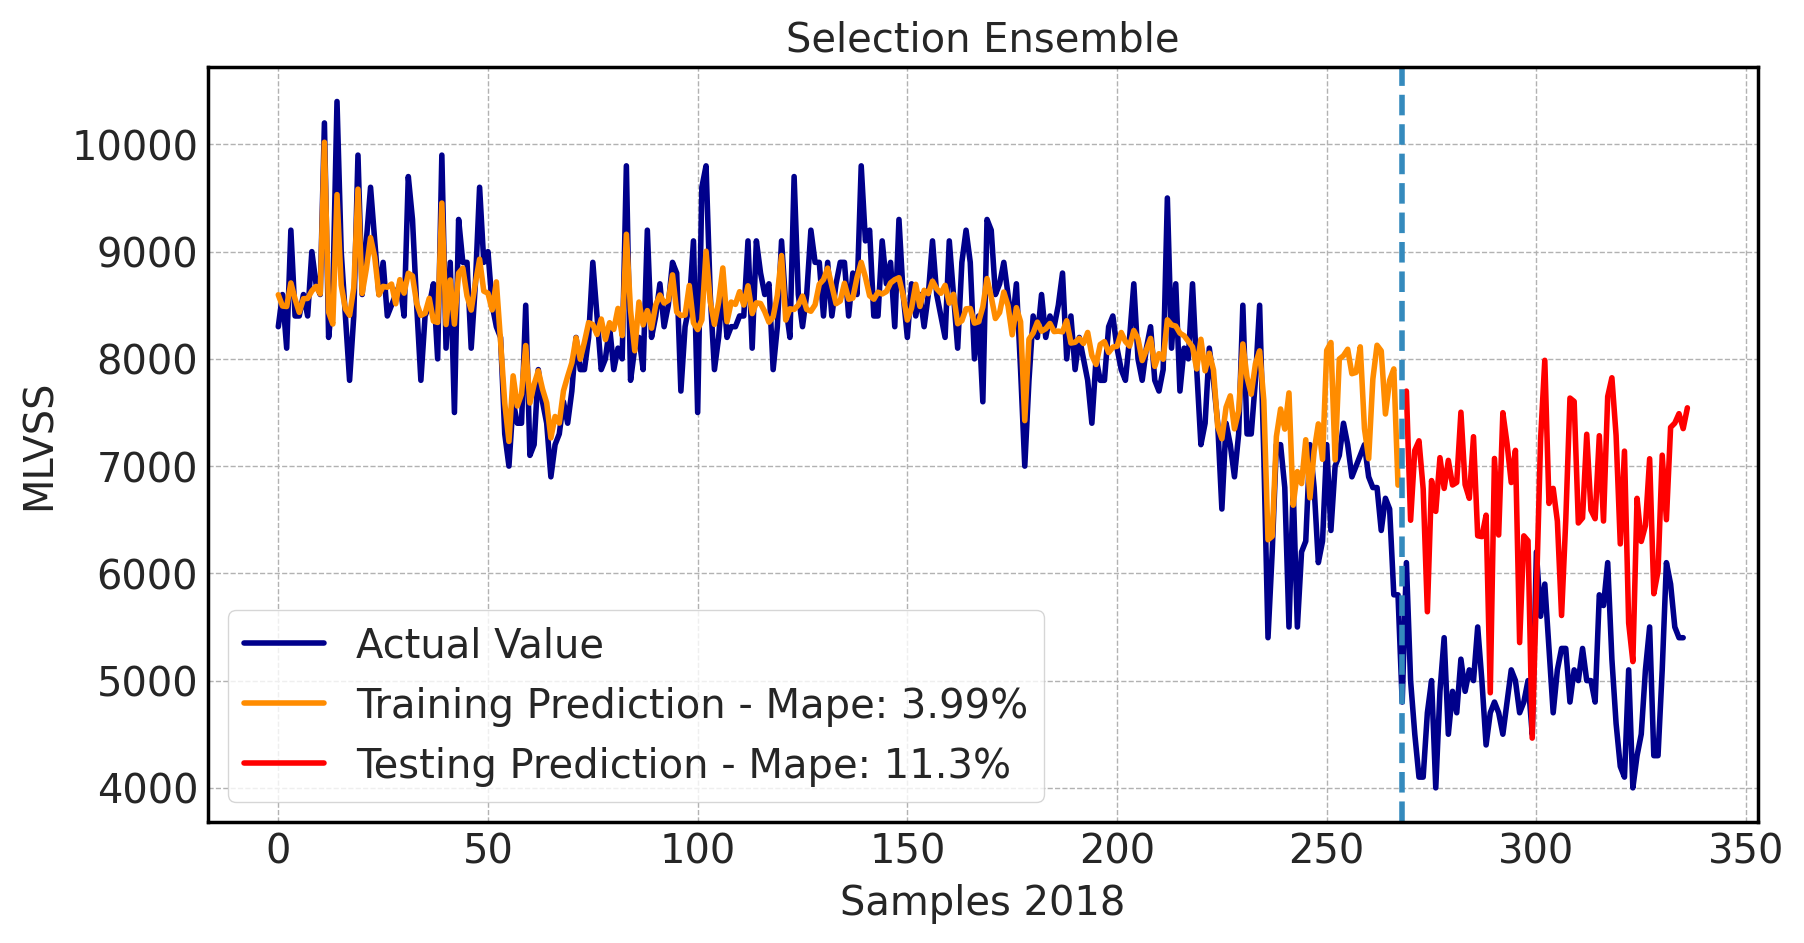
\includegraphics[width=\linewidth]{figures/test.png}
\caption{Approach 1 - MLVSS}
\label{f:App1-MLVSS}
\end{figure}

\section{Approach 2}
\label{s:Approach2}

The second approach uses a recurrent neural network, specifically a Long Short-Term Memory (LSTM), a powerful network architecture for sequential data which considers the effect of past values of both endogenous and exogenous variables by itself and learns possible time patterns during the training. Fig. 5 shows a general overview of the second approach. This network requires some data pre-processing to structure the data in sequences format (seven past steps are considered for this study), but nothing more than standardization is applied. 

\begin{figure}[h]
\centering
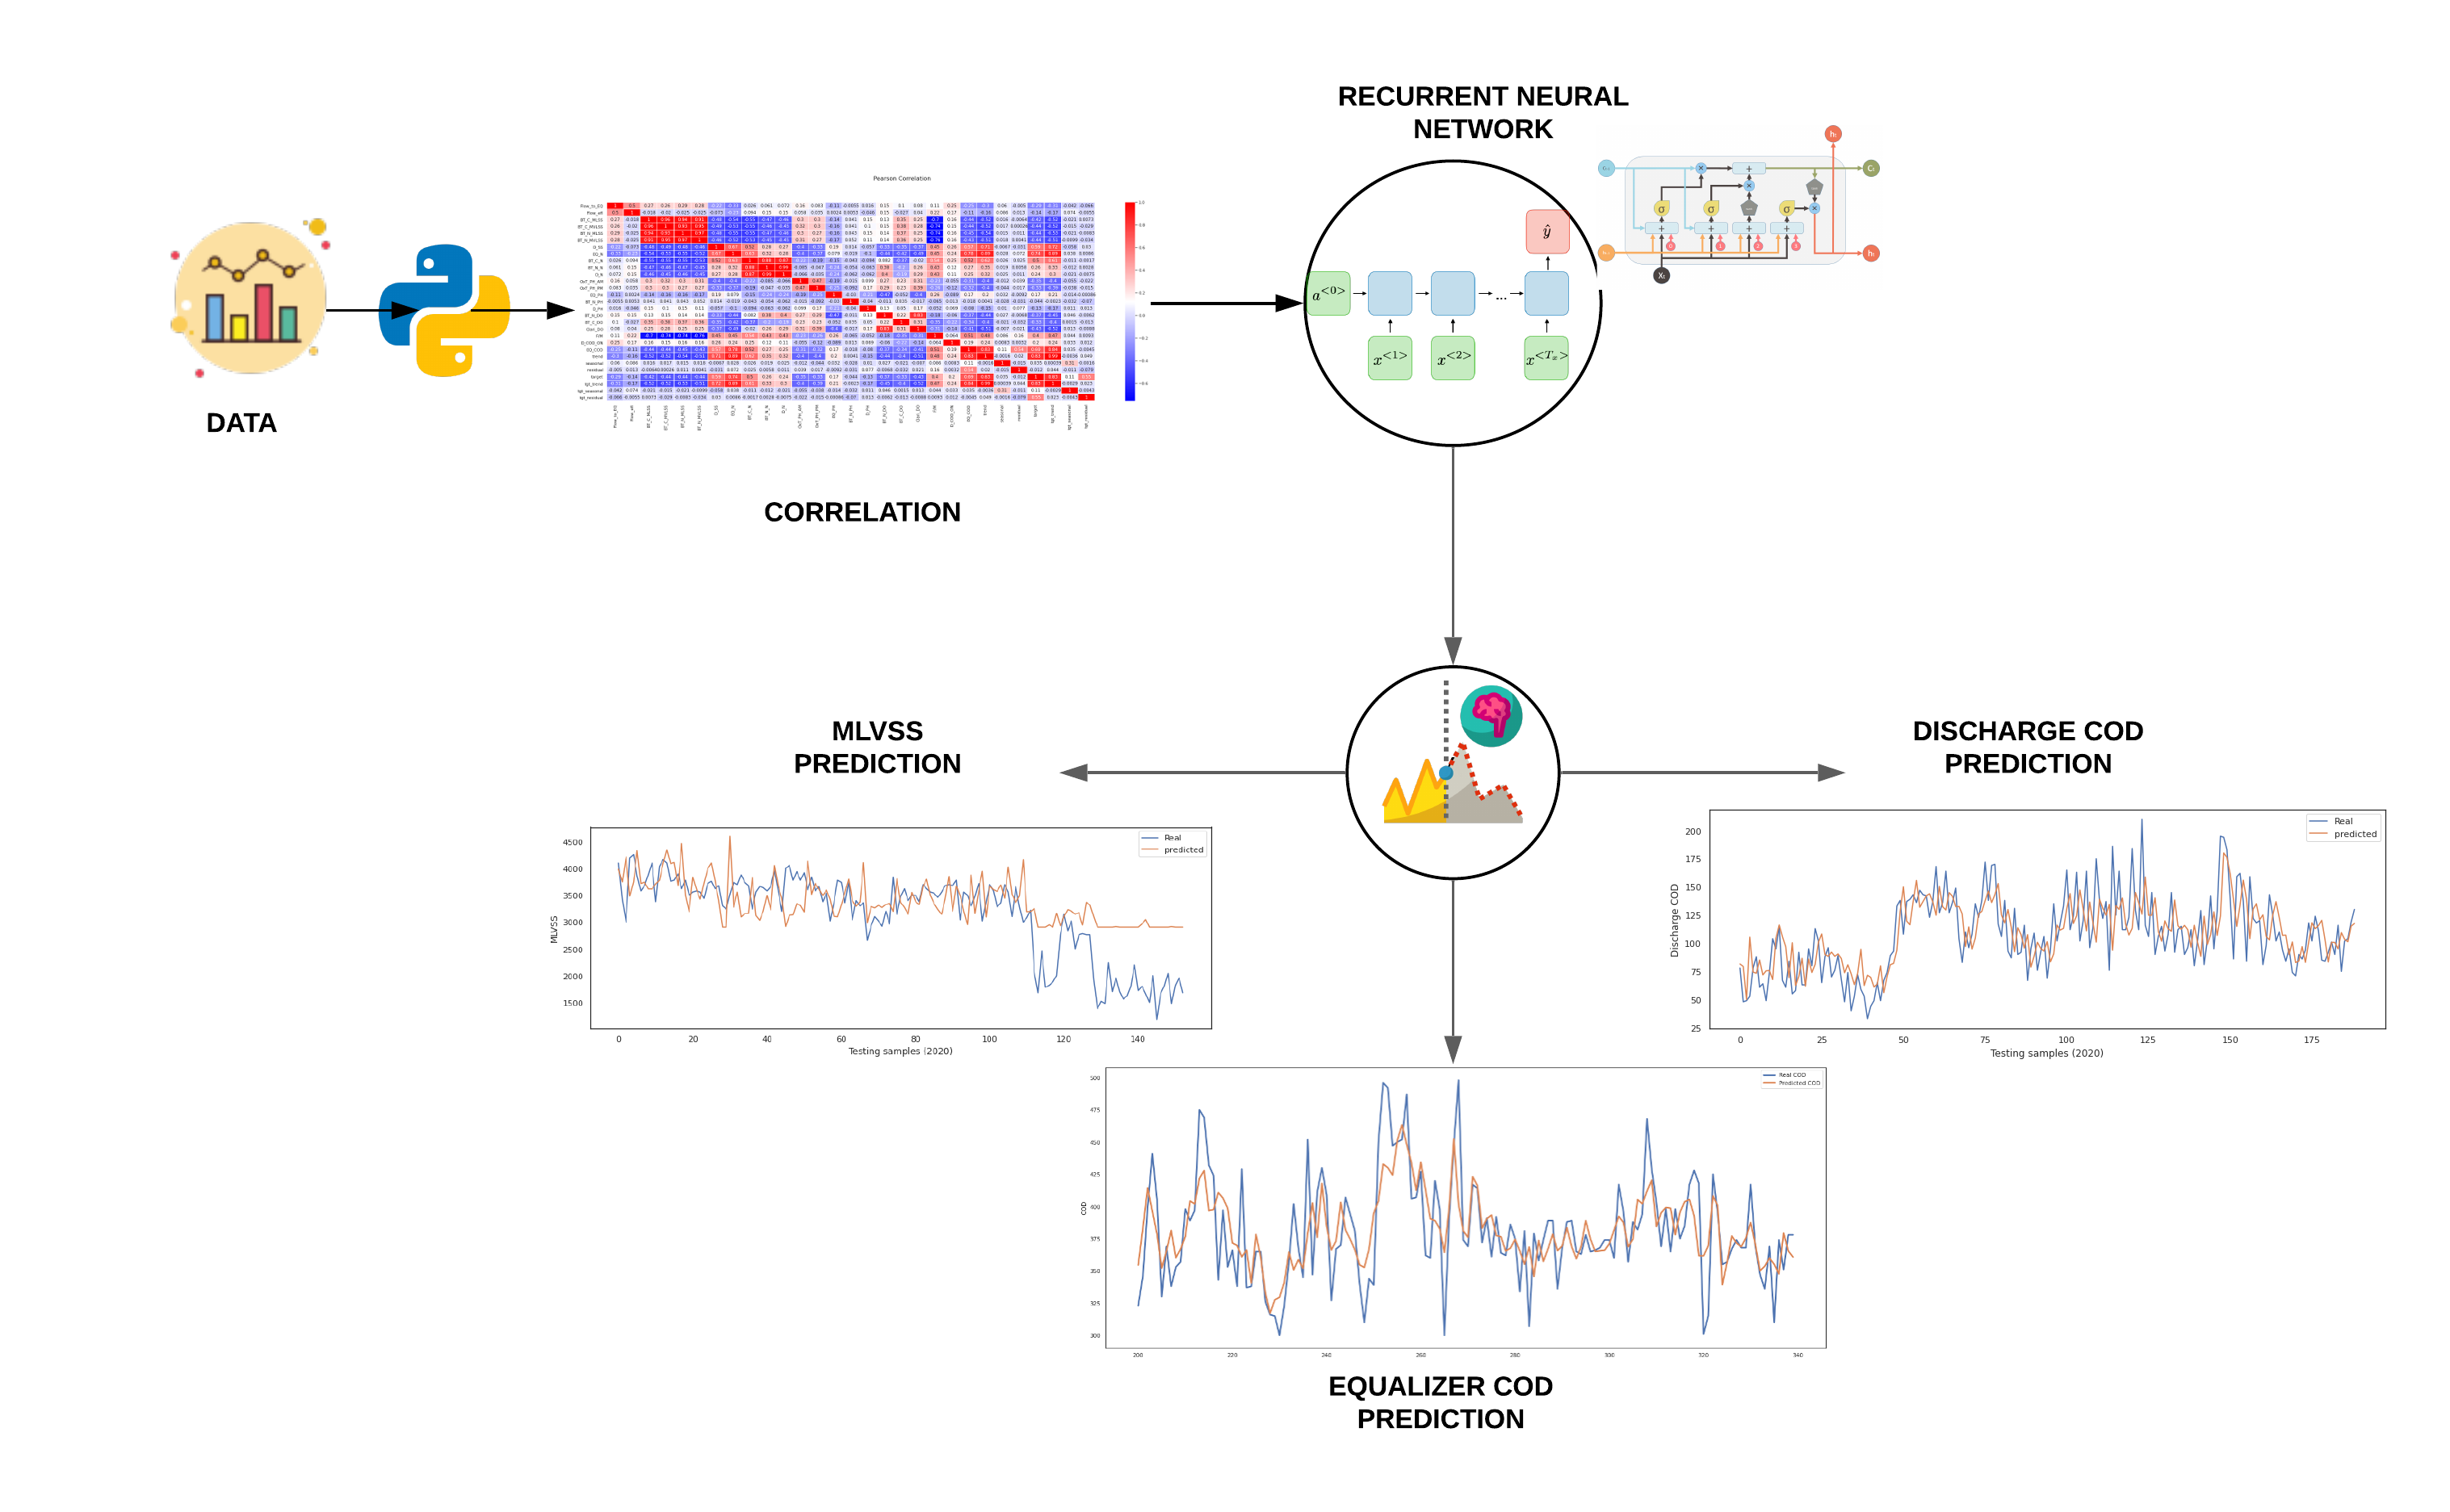
\includegraphics[width=\linewidth]{figures/Ch4/Approach2.png}
\caption{Approach 2}
\label{f:Approach 2}
\end{figure}

\begin{figure}[h]
\centering
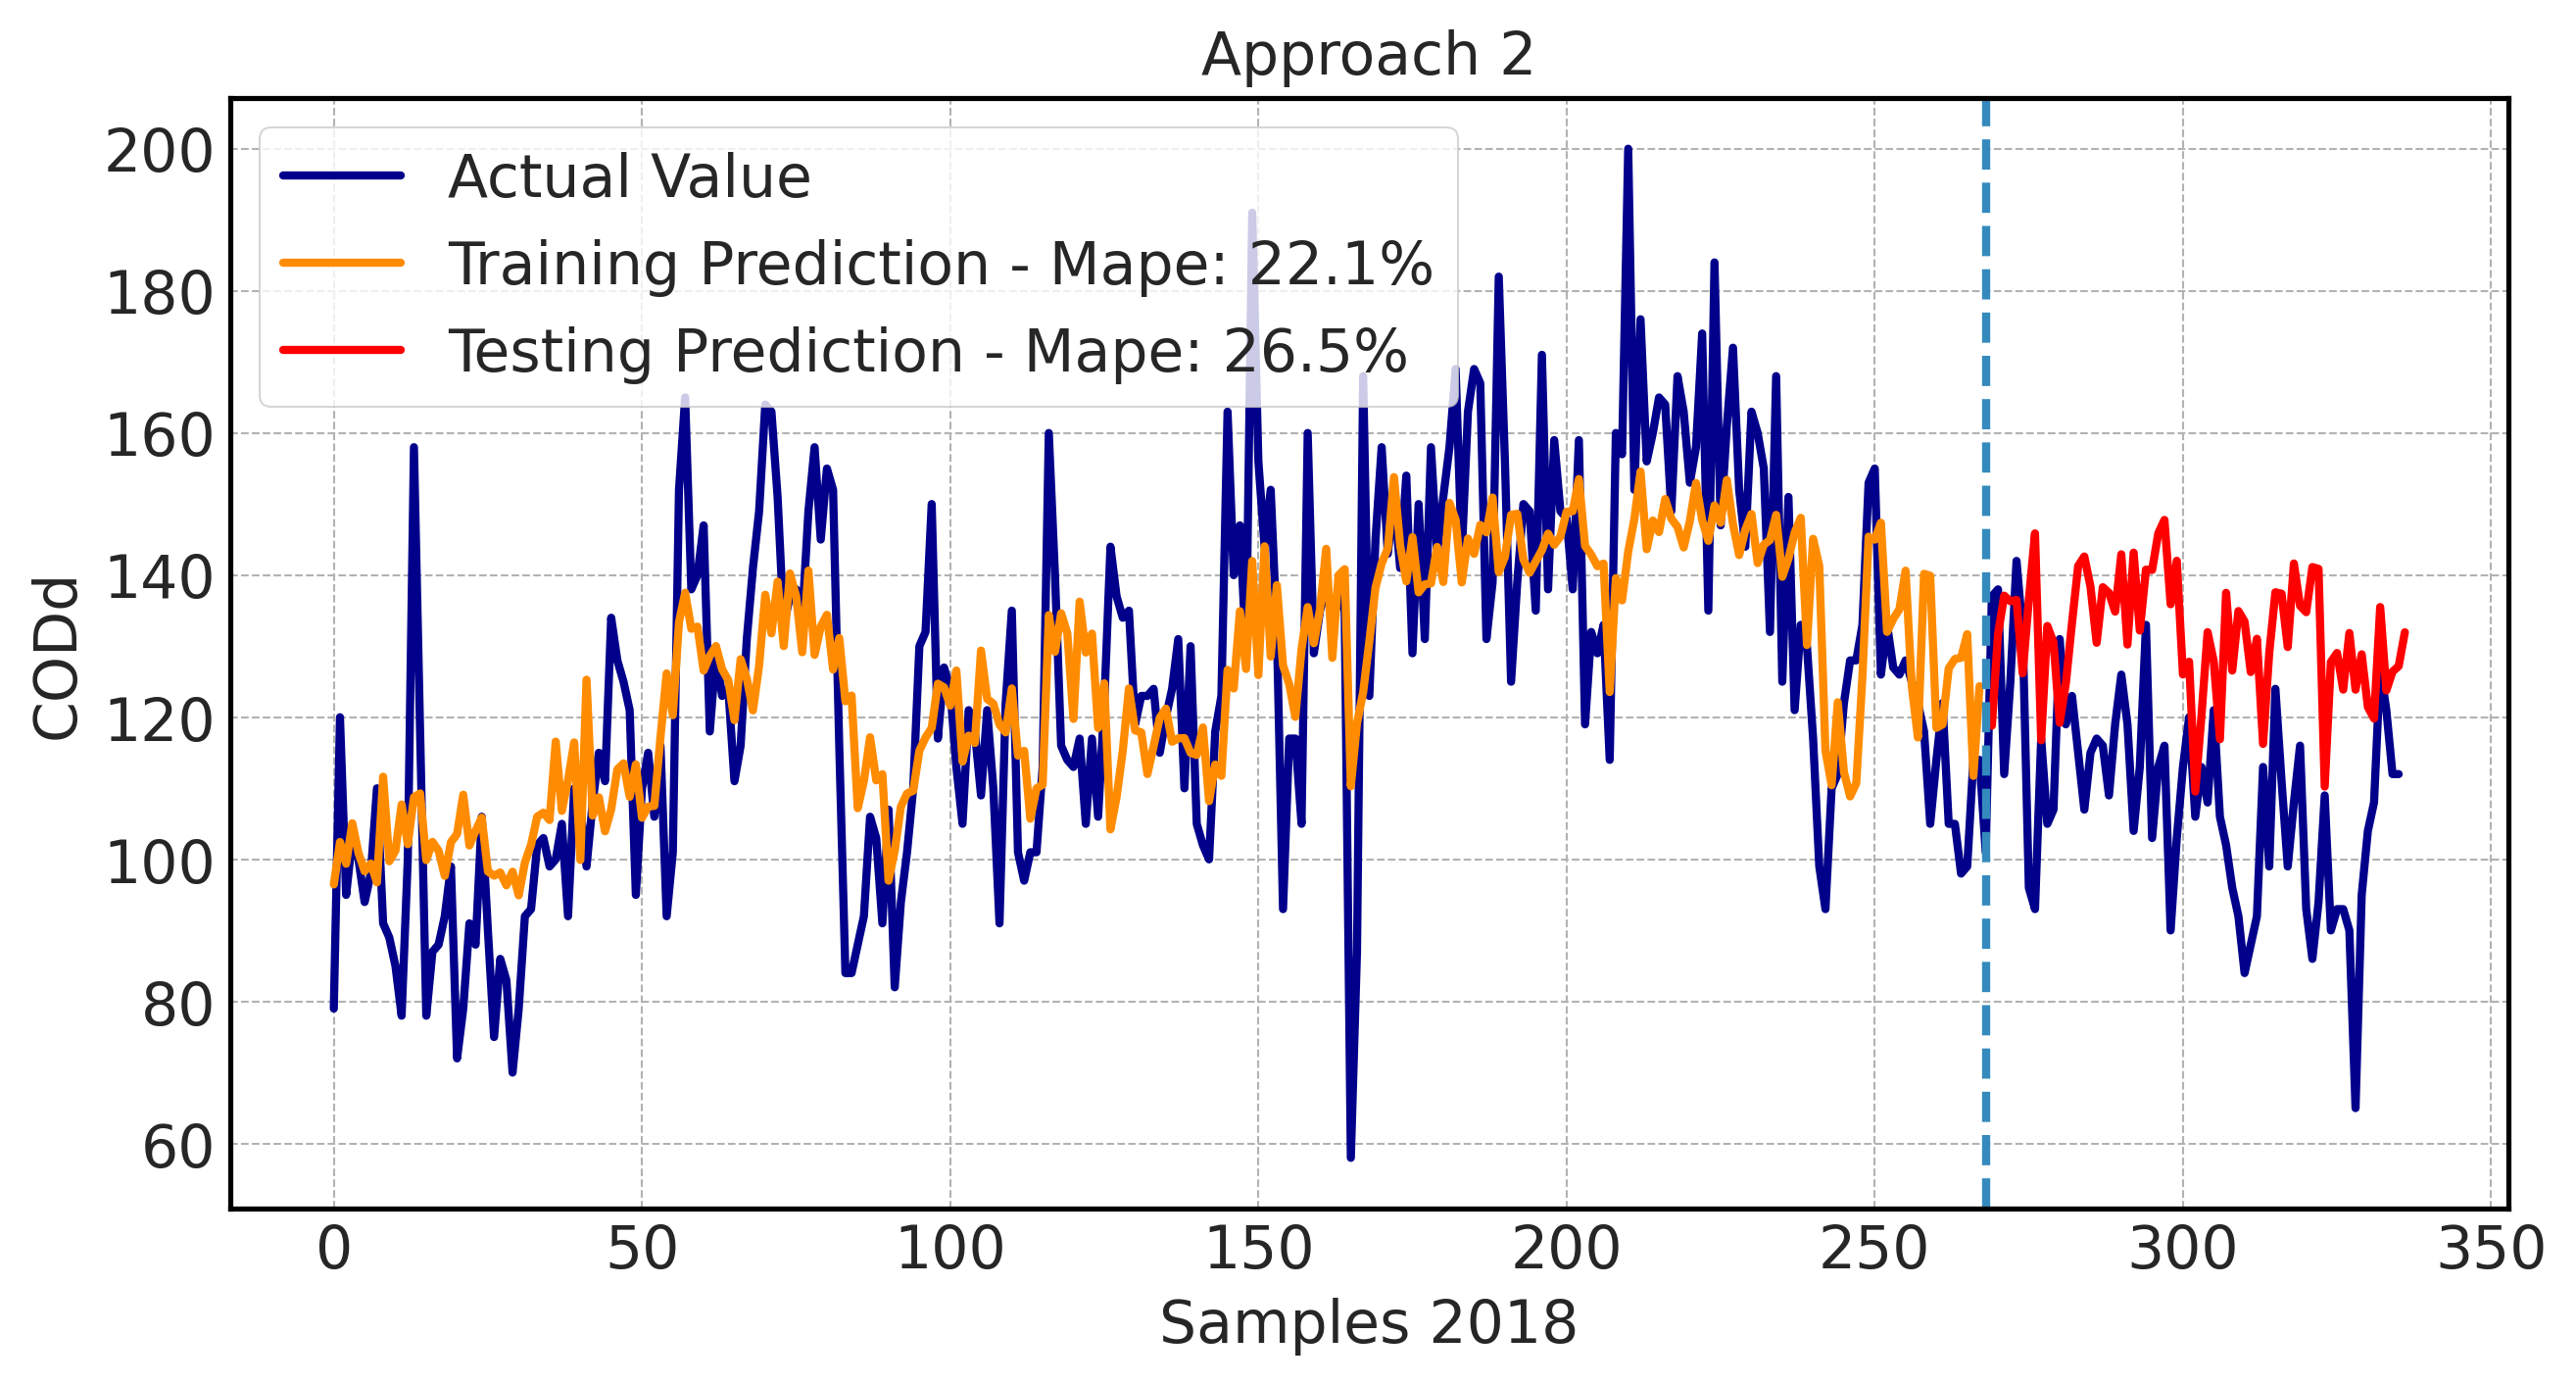
\includegraphics[width=\linewidth]{figures/Ch6/CODd-2.png}
\caption{Approach 2 - CODD}
\label{f:App2-codd}
\end{figure}

\begin{figure}[h]
\centering
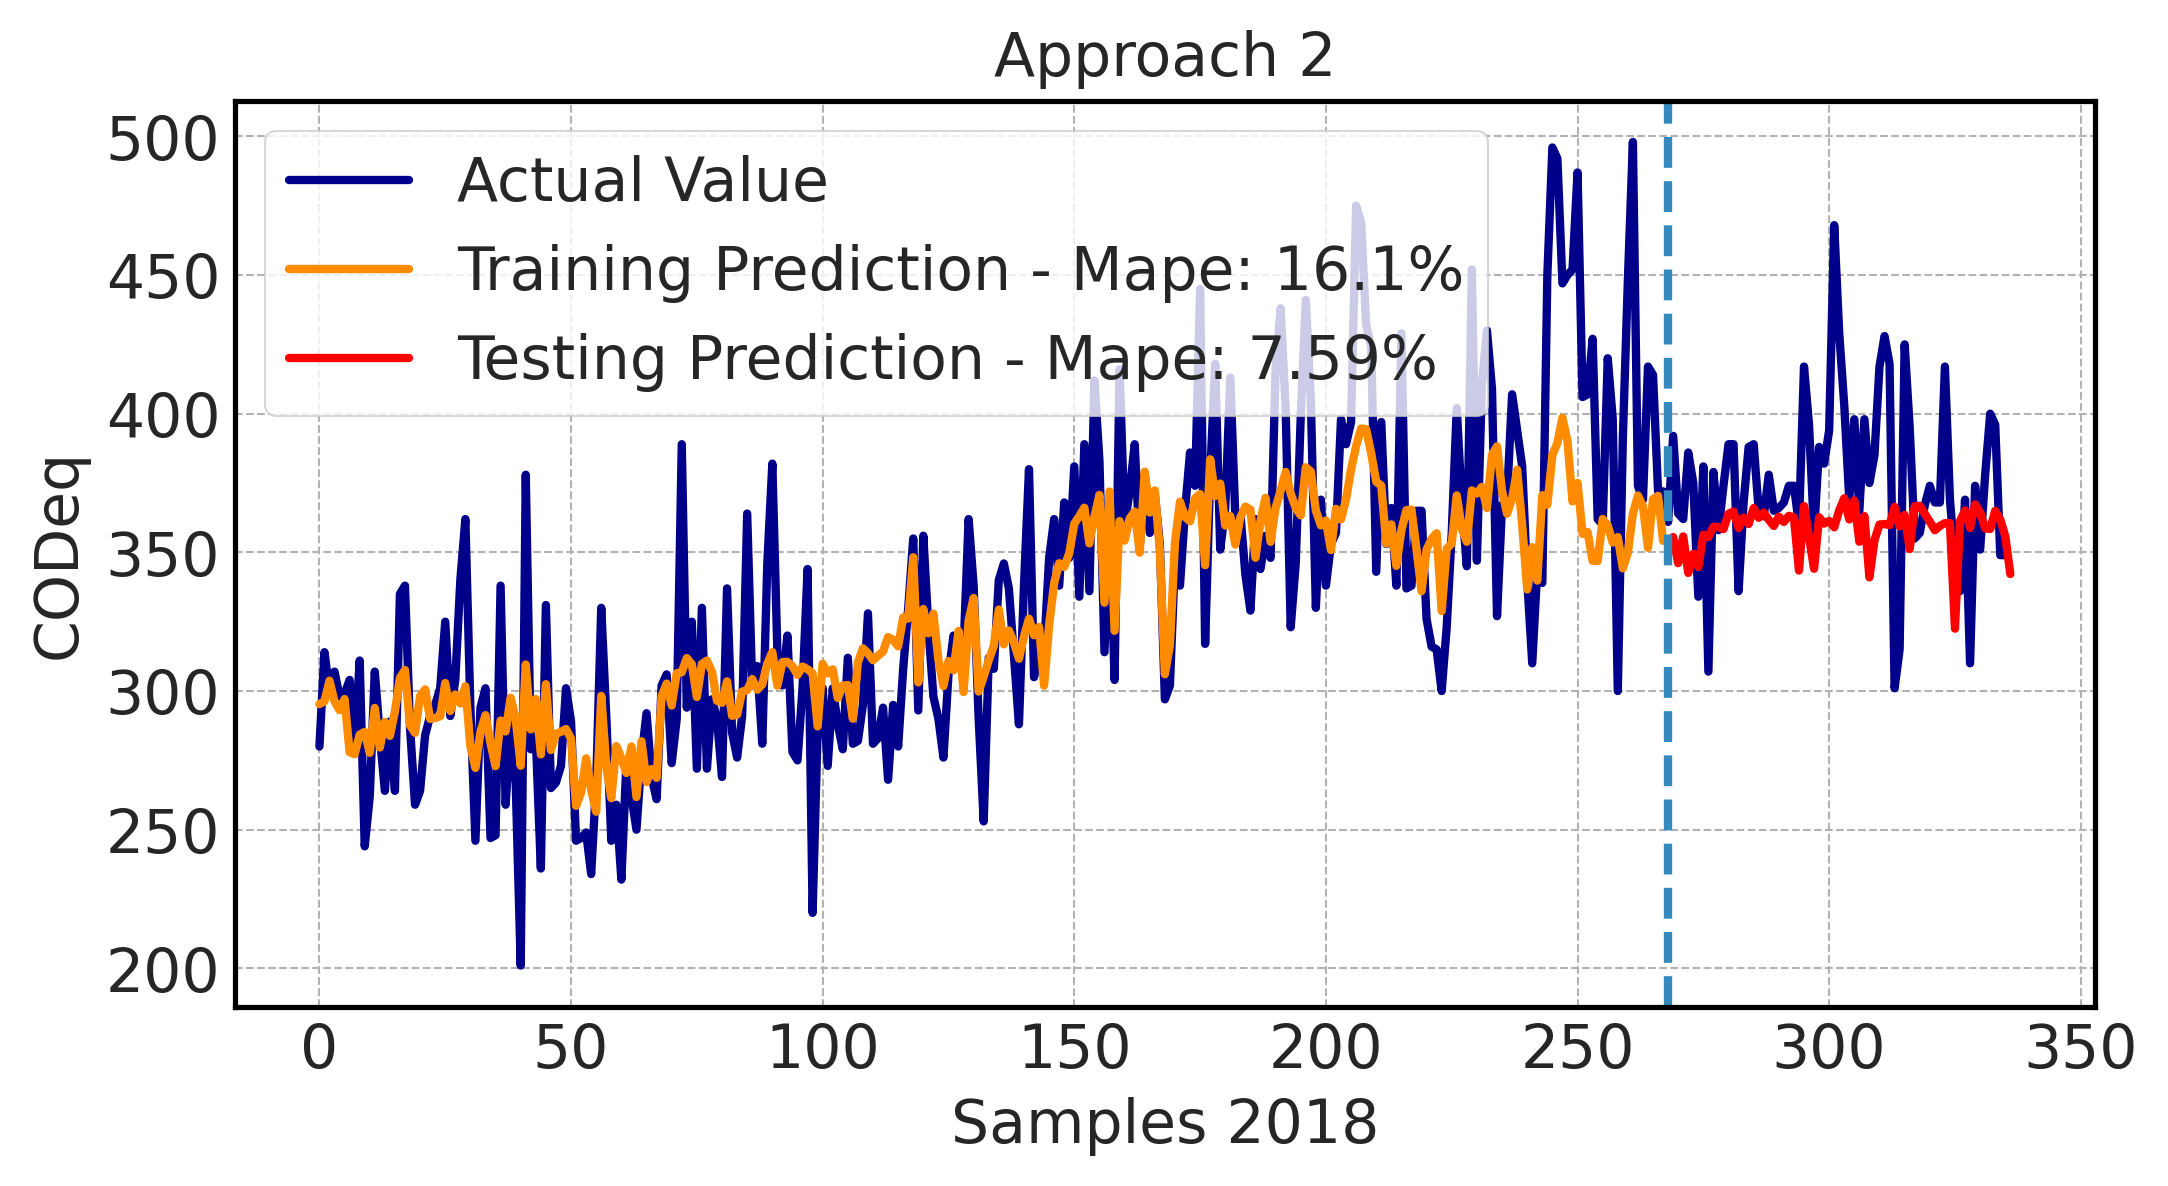
\includegraphics[width=\linewidth]{figures/Ch6/CODeq-2.png}
\caption{Approach 2 - CODEQ}
\label{f:App2-codeq}
\end{figure}

\begin{figure}[h]
\centering
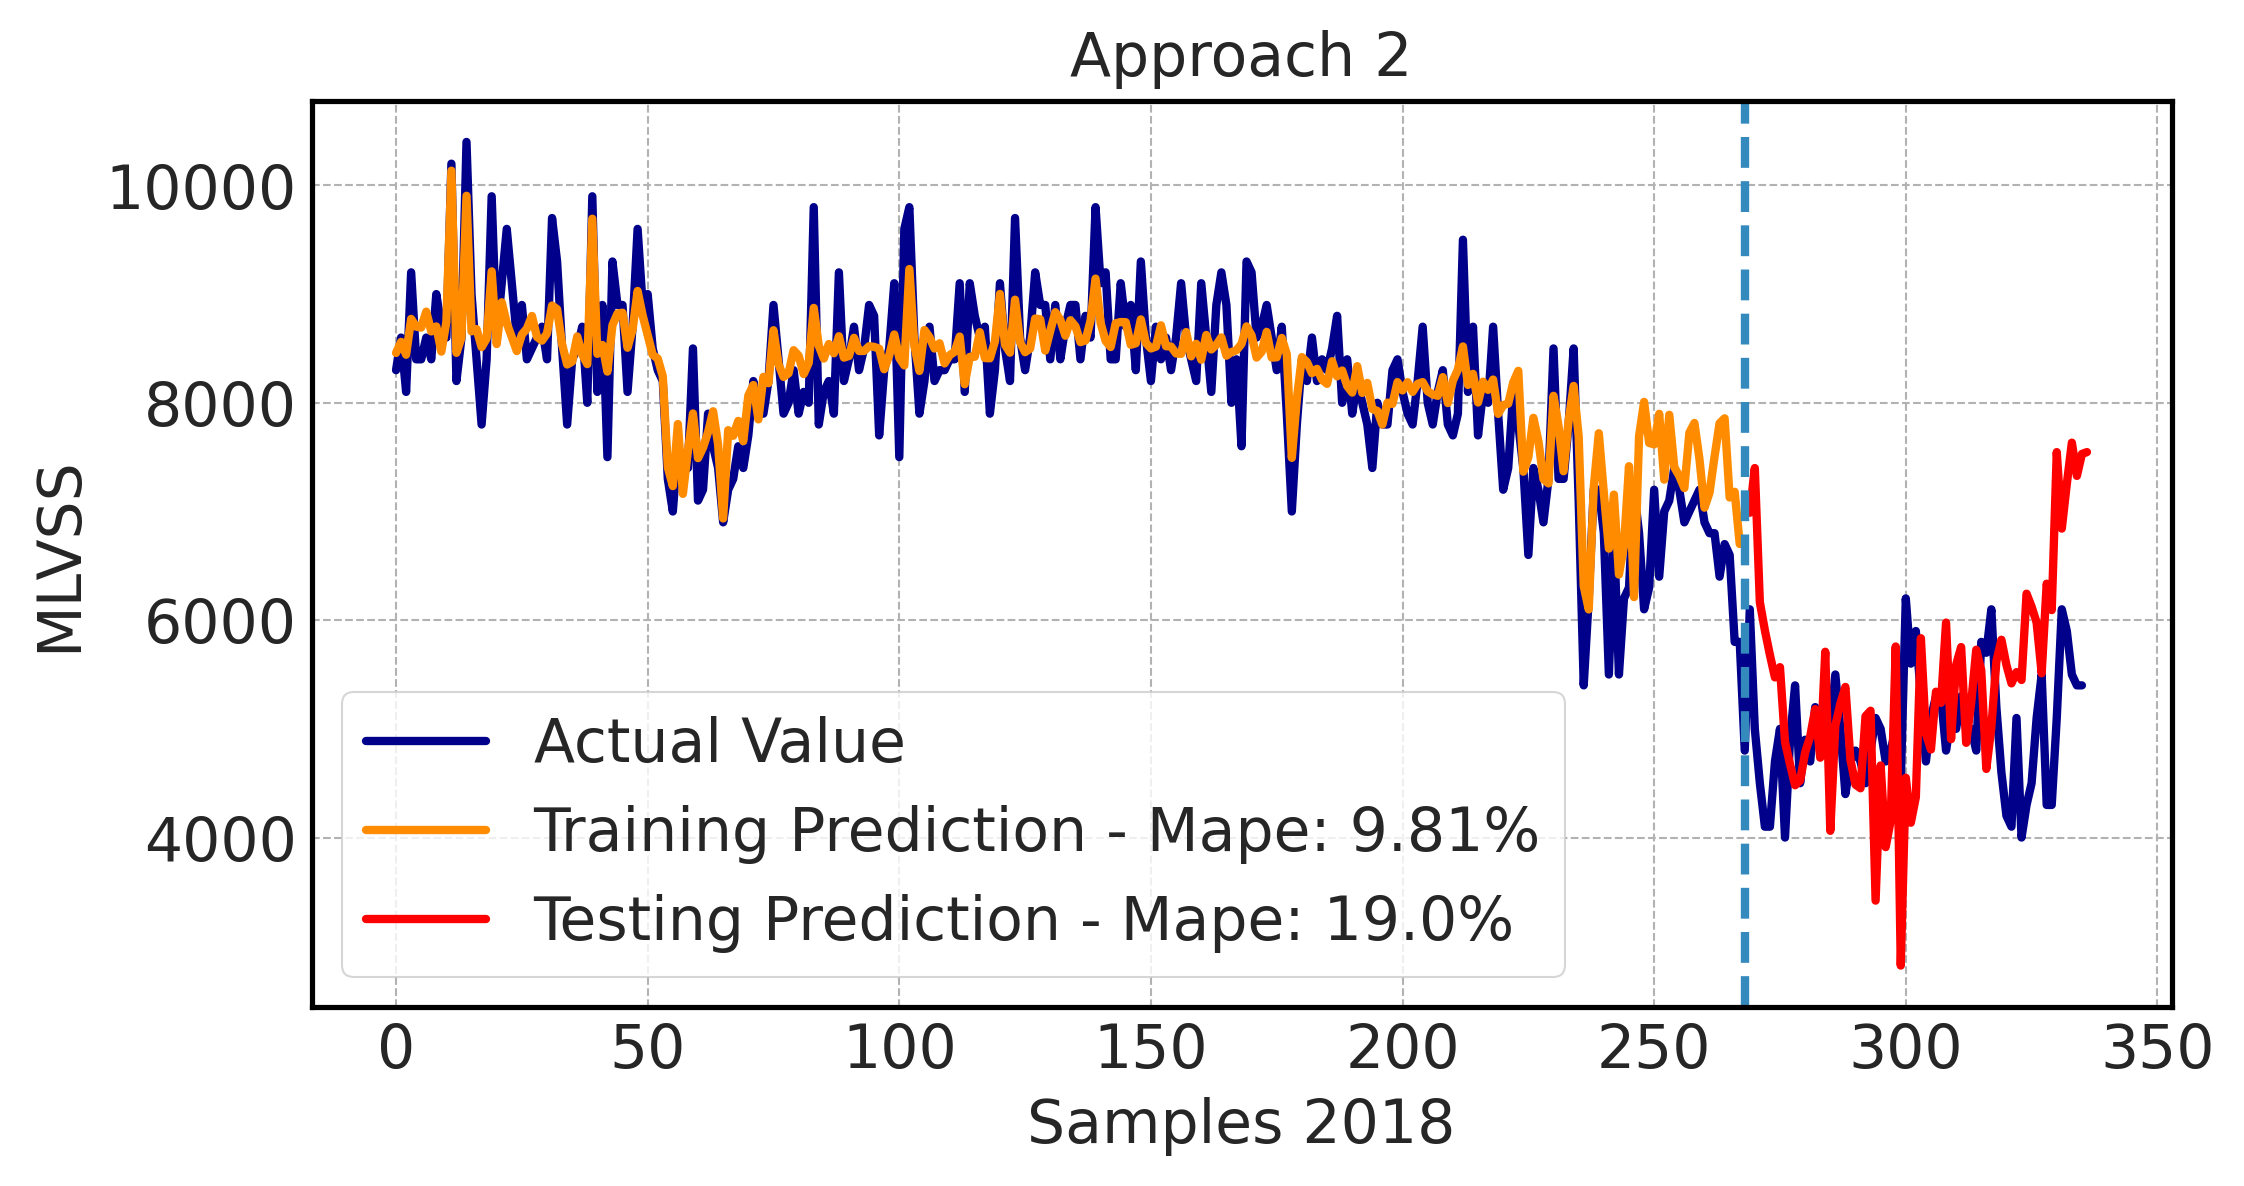
\includegraphics[width=\linewidth]{figures/Ch6/MVLSS-approach2.png}
\caption{Approach 2 - MLVSS}
\label{f:App2-MLVSS}
\end{figure}

\section{Approach 3}
\label{s:Approach3}

The third approach proposed uses a machine learning technique based on Support Vector Machines. The Support Vector Regression (SVR) algorithm offers an accurate prediction of the time series. This model receives as inputs the exogenous variables selected from the correlation analysis. The implemented model uses Radial Base Function (RBF) kernel, gamma of 0.001, epsilon equal to 0.2 and c value of 10.

\begin{figure}[h]
\centering
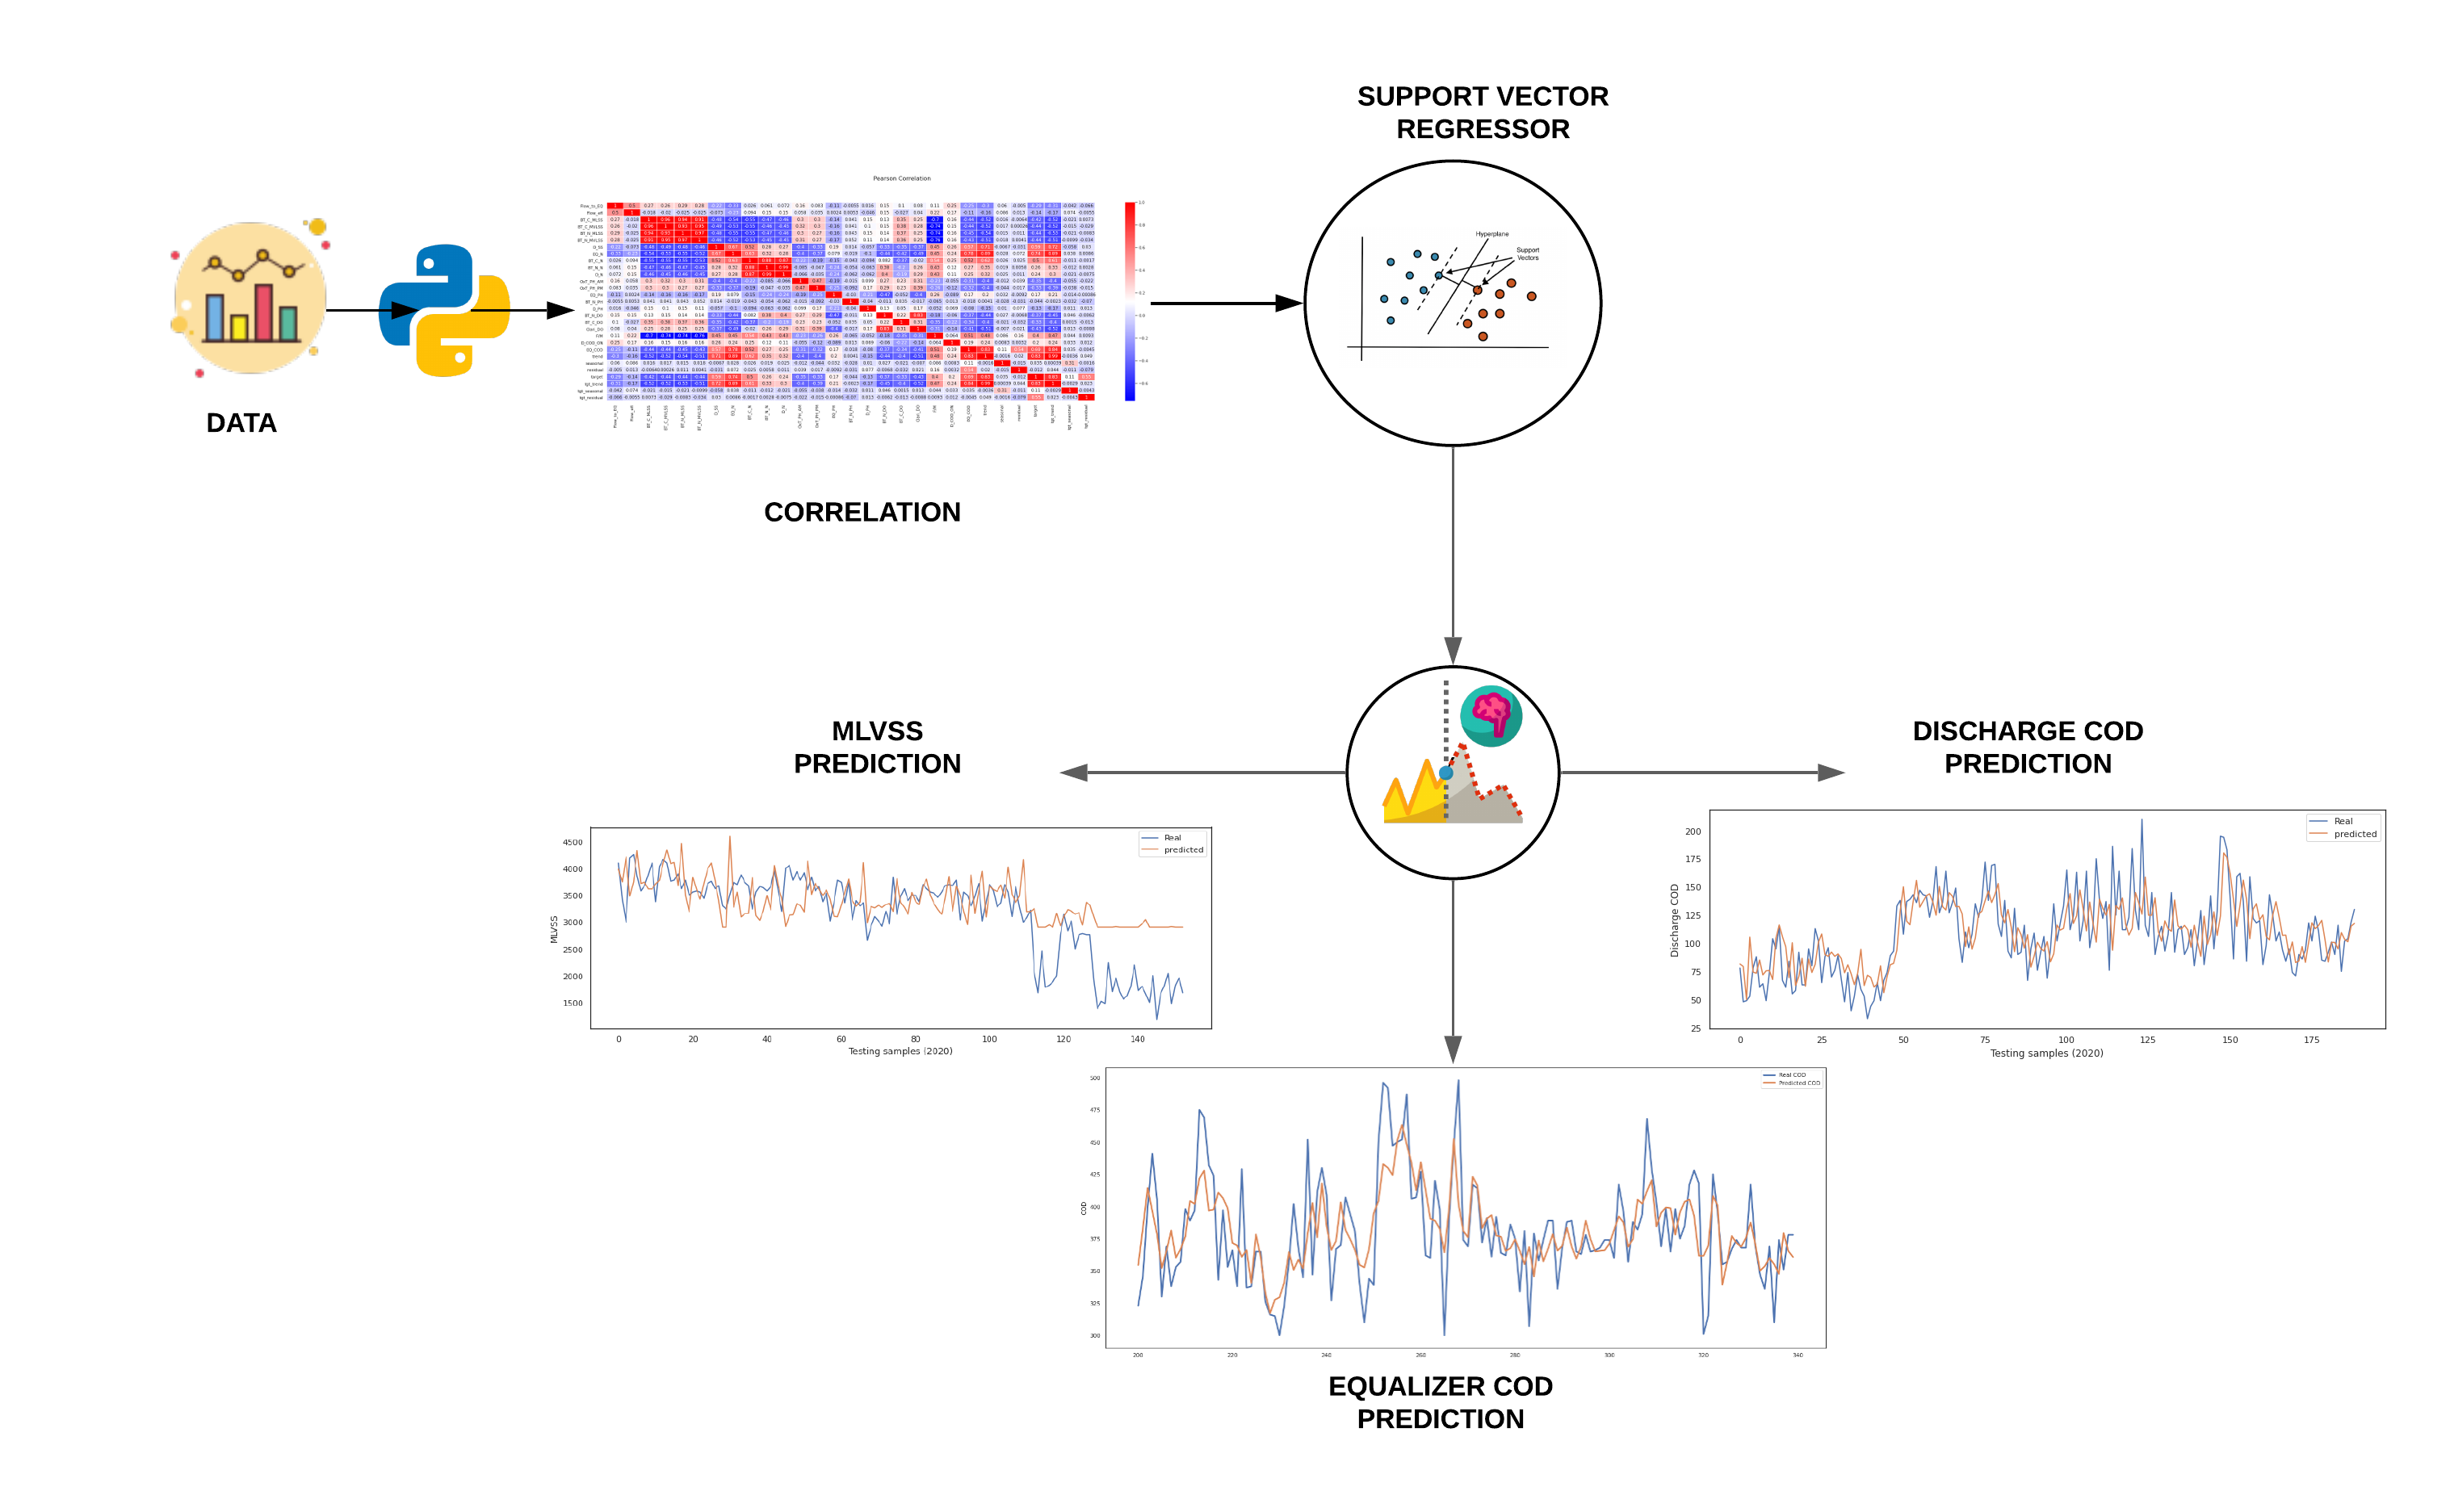
\includegraphics[width=\linewidth]{figures/Ch4/Approach3.png}
\caption{Approach 3}
\label{f:Approach 3}
\end{figure}

\begin{figure}[h]
\centering
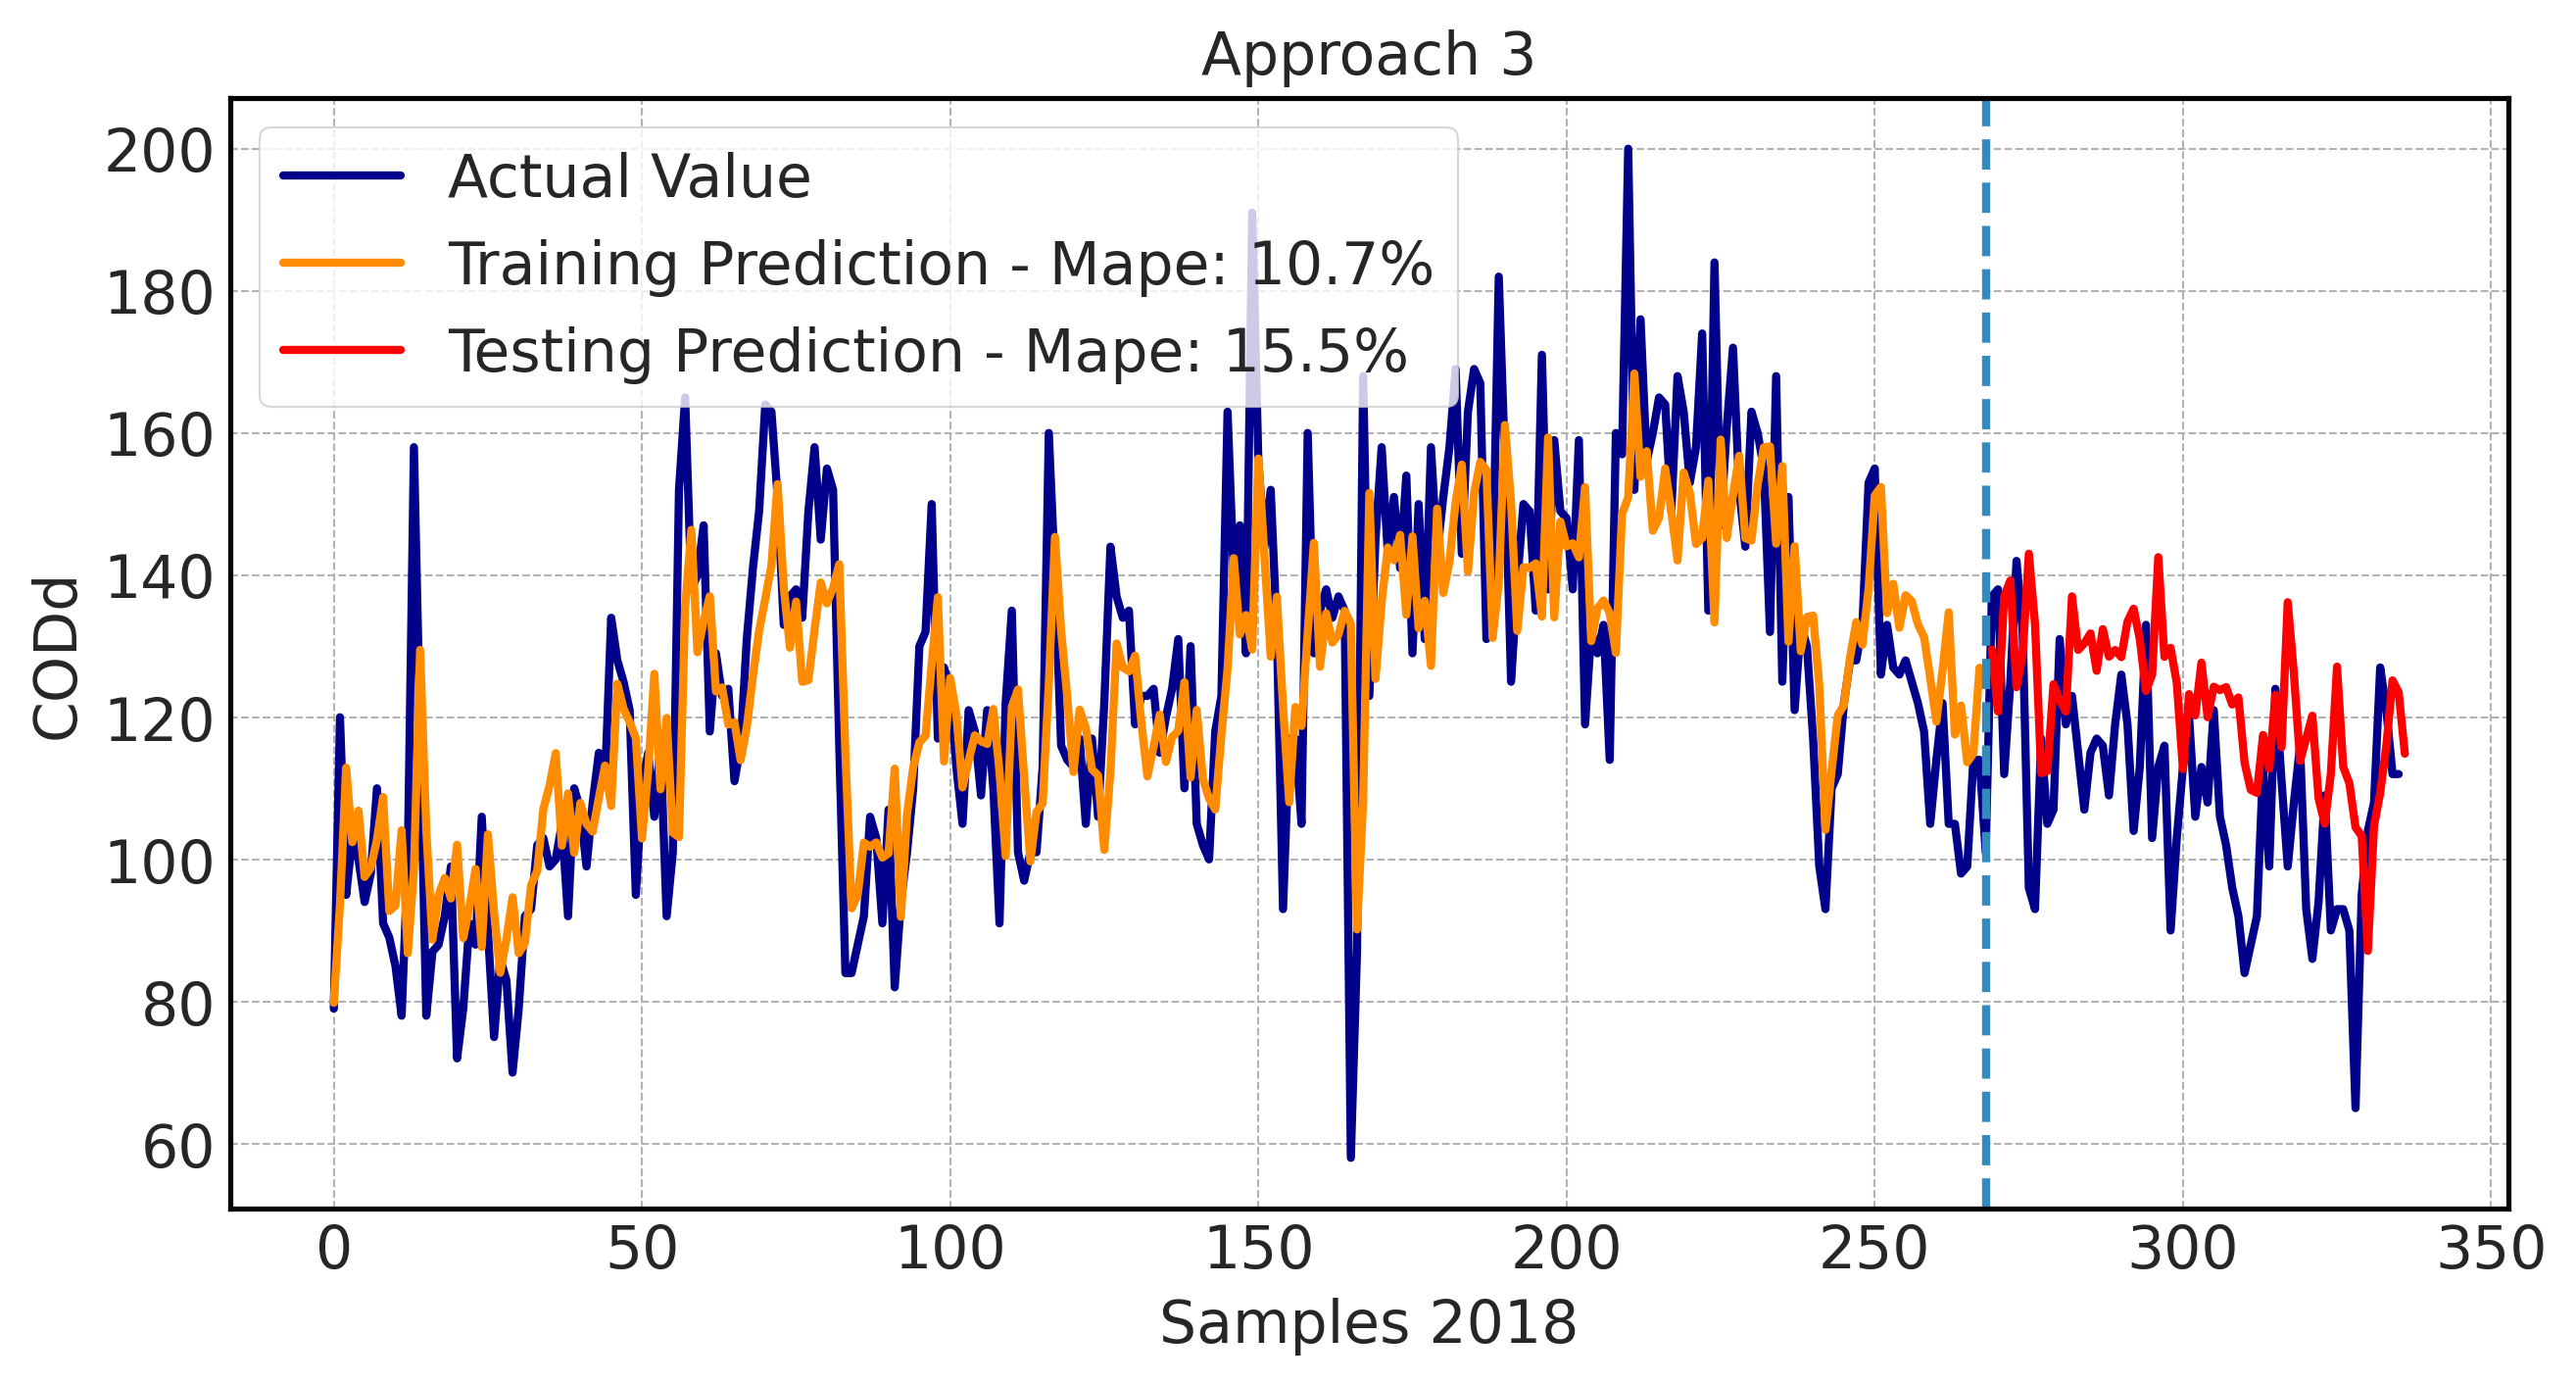
\includegraphics[width=\linewidth]{figures/Ch6/CODd-3.png}
\caption{Approach 3 - CODD}
\label{f:App3-codd}
\end{figure}

\begin{figure}[h]
\centering
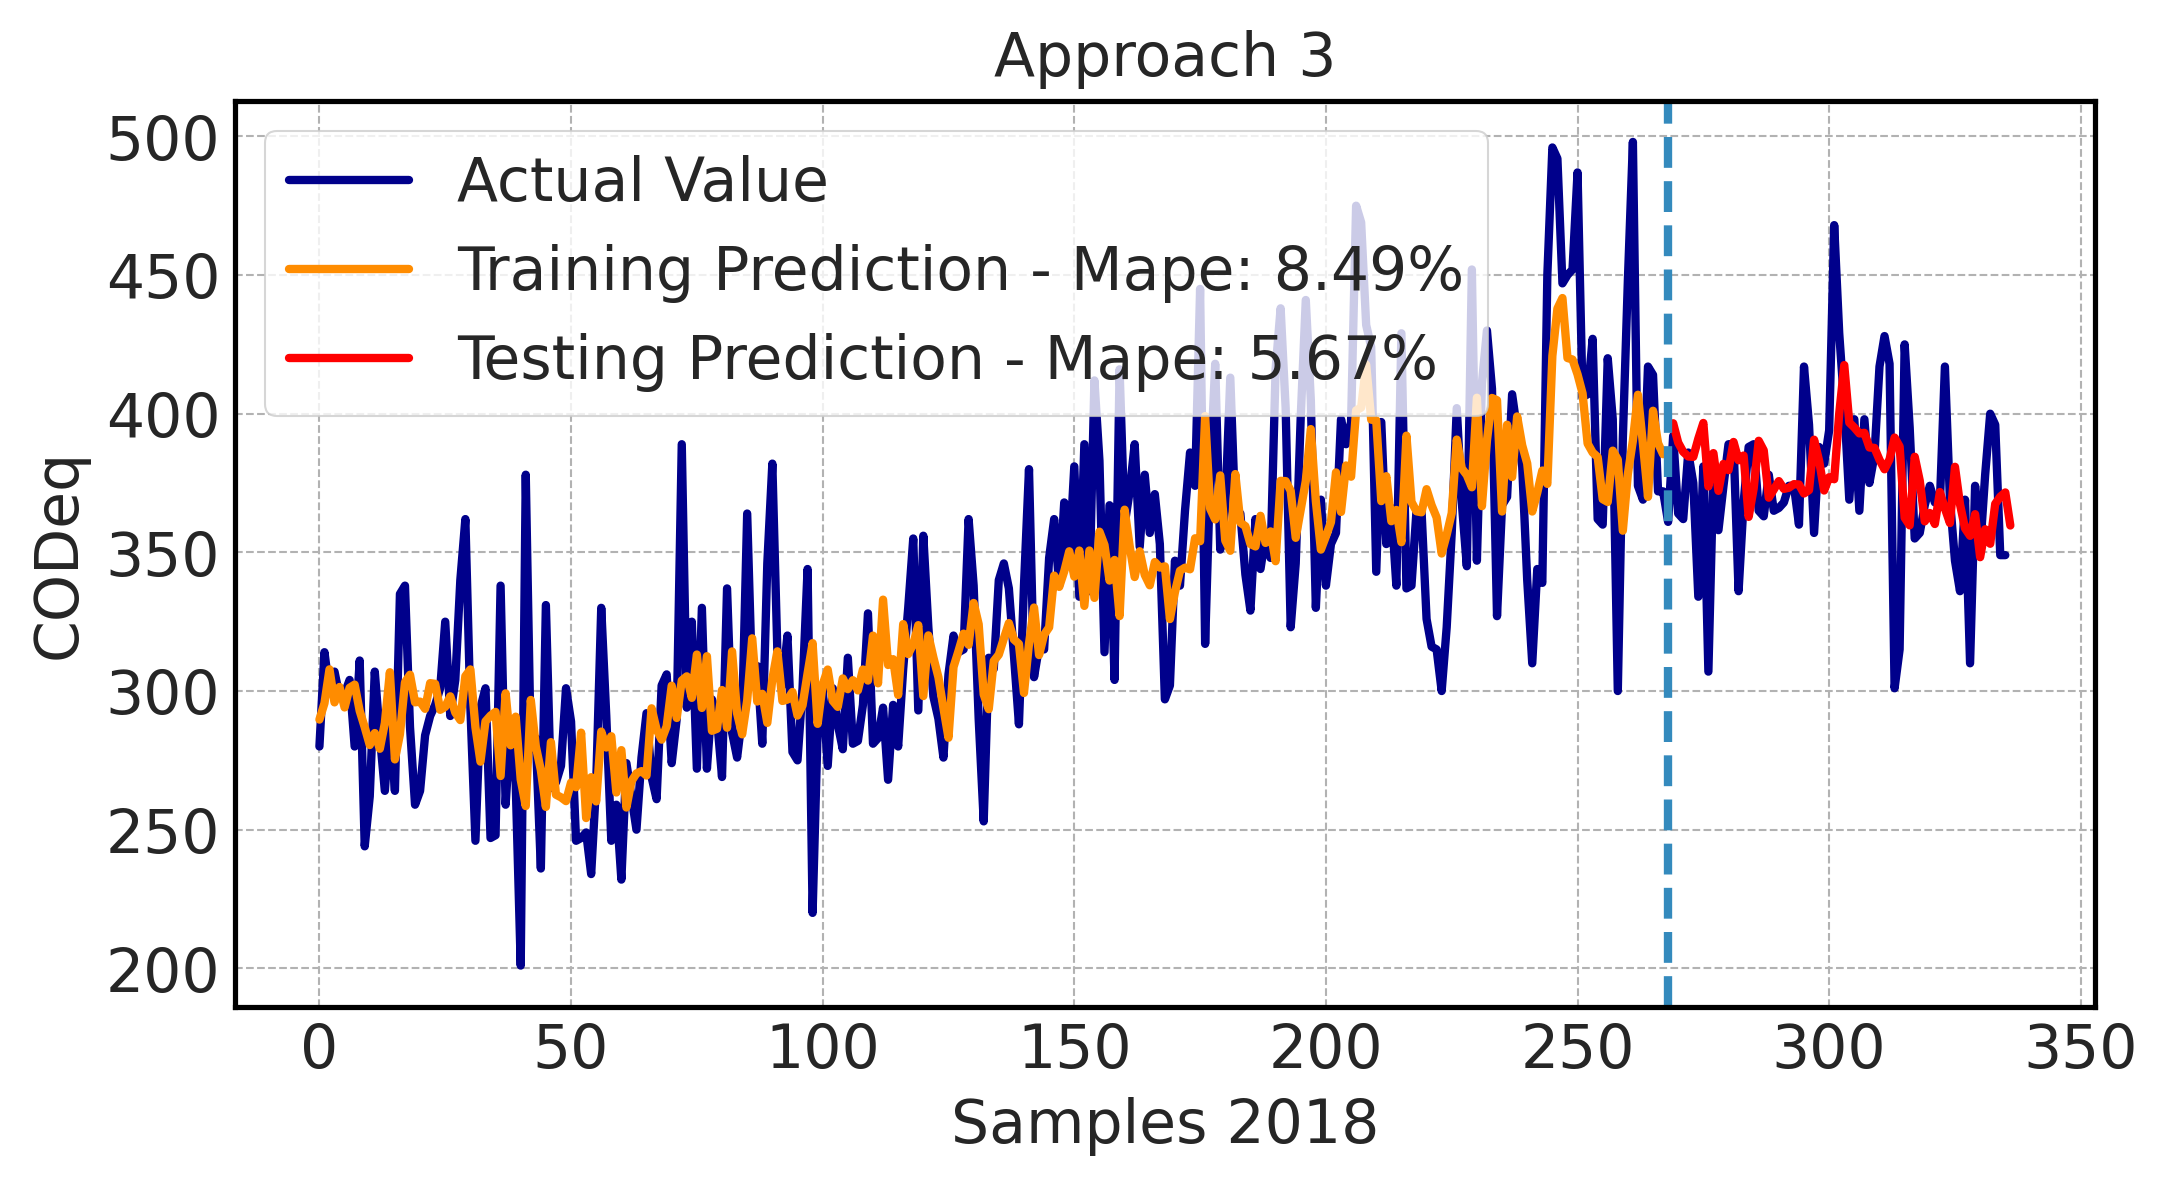
\includegraphics[width=\linewidth]{figures/Ch6/CODeq-3.png}
\caption{Approach 3 - CODEQ}
\label{f:App3-codeq}
\end{figure}

\begin{figure}[h]
\centering
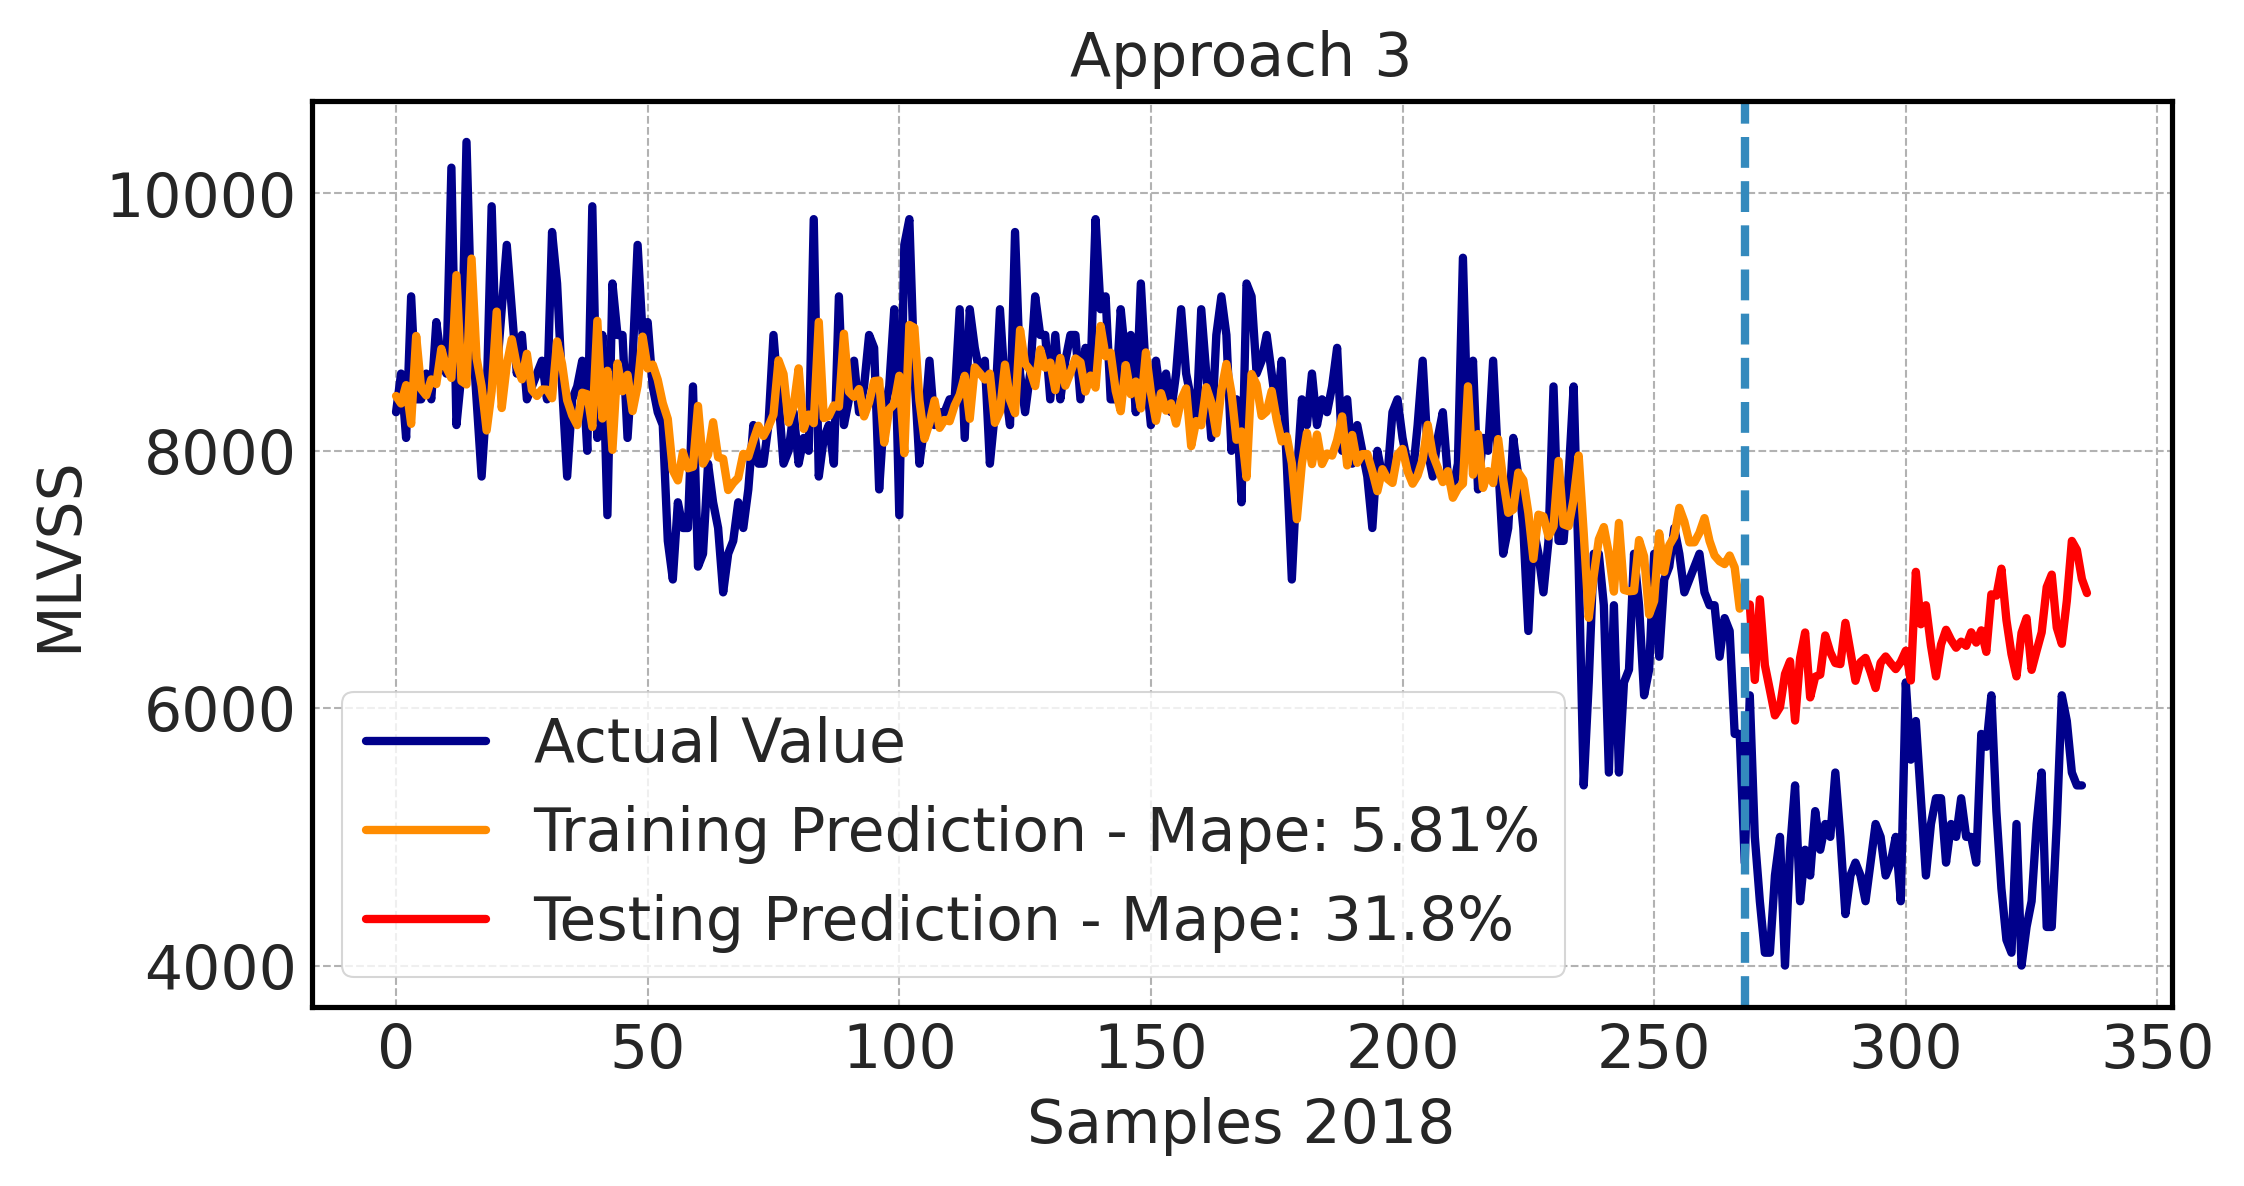
\includegraphics[width=\linewidth]{figures/Ch6/MVLSS-approach3.png}
\caption{Approach 3 - MLVSS}
\label{f:App3-MLVSS}
\end{figure}


\section{Summary}
\label{s:Contribution-1-Summary}

The final section of each major chapter should summarize the chapter. In comparison to the chapter, the summary should be short ($\frac{1}{2}$ to $2$ pages is normal).